\documentclass[12pt]{report}
\usepackage[utf8]{inputenc}
\usepackage{tabularx} % extra features for tabular environment
\usepackage{amsmath,amssymb,amsthm}  % improve math presentation
\usepackage[ruled,vlined]{algorithm2e}
\usepackage{caption}
\usepackage{subcaption}
\usepackage[hyphens]{url}
\usepackage[toc,page]{appendix}
\newcommand{\E}{\mathrm{E}}
\newcommand{\Var}{\mathrm{Var}}
\newcommand{\Cov}{\mathrm{Cov}}
\newcommand{\Cor}{\mathrm{Cor}}
\DeclareMathOperator*{\argmin}{argmin}
\DeclareMathOperator*{\argmax}{argmax}
\newcommand\norm[1]{\left\lVert#1\right\rVert}
\newcommand\myleqa{\mathrel{\overset{\makebox[0pt]{\mbox{\normalfont\tiny\sffamily (a)}}}{\leq}}}
\newcommand\myleqb{\mathrel{\overset{\makebox[0pt]{\mbox{\normalfont\tiny\sffamily (b)}}}{\leq}}}
\newcommand\myleqc{\mathrel{\overset{\makebox[0pt]{\mbox{\normalfont\tiny\sffamily (c)}}}{\leq}}}
\newcommand\myeqa{\mathrel{\overset{\makebox[0pt]{\mbox{\normalfont\tiny\sffamily (a)}}}{=}}}
\newcommand\myeqb{\mathrel{\overset{\makebox[0pt]{\mbox{\normalfont\tiny\sffamily (b)}}}{=}}}
\usepackage{graphicx} % takes care of graphic including machinery
\usepackage{cite}
\usepackage[margin=1in,letterpaper]{geometry} % decreases margins
\usepackage[final]{hyperref} % adds hyper links inside the generated pdf file
\hypersetup{
	colorlinks=true,       % false: boxed links; true: colored links
	linkcolor=black,        % color of internal links
	citecolor=black,        % color of links to bibliography
	filecolor=magenta,     % color of file links
	urlcolor=black         
}
\usepackage{setspace}
\doublespacing

\begin{document}

\title{
{
\includegraphics[width=0.7\columnwidth]{university.jpg}}\\
{Greedy Principal Flows}\\
{\large National University of Singapore}\\
}
\author{Sebastian Lie}
\date{05 March 2021}
\maketitle

\chapter*{Acknowledgements}
First and foremost I would like to thank my supervisor, Prof Yao Zhigang
for his invaluable guidance and insight throughout this project. This report
and my results would not be the way it is if not for him. To my friends
from both Science and Computing: thank you for your companionship, 
the jokes that keep me amused, and help in the 
modules we have taken together. You make my days that much brighter. 
To my friends from CAPT: thank you for the wonderful, thought-provoking conversations,
the laughter and the warmth you all bring to my life. 
Staying in CAPT has been one of the best decisions I have ever made.
To my friends from CJC: thank you all for making me laugh so hard and for being 
a source of comfort. I always look forward to our meet-ups and I always laugh so 
effortlessly around you all.
To Marcus: for being a loveable idiot that has kept me sane through my years schooling. 
Thank you for being the brother I never had.
To my parents: thank you for your unwavering support, advice, love and food.
These have been my fuel for the last few months. 
To Gek: thank you for being a constant who brings much light, warmth and 
happiness to my life. You are the 
lighthouse that guides me to shore amongst the stormy seas. 
Last but definitely not least, I dedicate this to God, the Rock in whom I trust. 
Through Him all things are possible.


\chapter*{Abstract}

Principal Flows are a great tool to use when we want to extend the 
notion of Principal Component Analysis to multivariate high dimensional data that 
lie on non-linear lower dimensional manifolds.
This is especially since principal flows are curves on a manifold 
that move along a path of maximal variation of the data, and capture patterns of
variation that would escape Principal Component Analysis.
Principal flows were originally obtained by solving a problem
in variational calculus using the Euler-Lagrange method. 
In this thesis, we explore the use of a novel, simpler approach to constructing 
principal flows: a greedy approach.
Furthermore, since after rotation, centering, translation 
and normalisation, vectors can be viewed as points on the hypersphere, 
we restrict this problem to constructing principal flows on hypersphere.
Let us call this new approach the greedy principal flow.
We test the effectiveness of our greedy principal flow on toy data, and
explore the patterns of variation it finds in real world data. Our results show that
our greedy principal flow retains the same effectiveness as the original, and
finds meaningful patterns in existing real world data.

\newpage
\tableofcontents
\listoffigures
\newpage

\chapter{Introduction}

\section{Motivation}

With the advent of Big Data, and massive improvements in computing,
machine learning has been used successfully to solve a variety of problems, 
such as regression and classification problems. However, machine learning
can also be used in a more subtle, but no less important way: to discover patterns
in the data and glean more information from it. Among methods that have this aim, 
Principal Component Analysis (PCA) is the most popular and 
commonly taught. It does however, have a glaring weakness: it does 
not perform well when the data we are working with is sampled from a non-linear manifold.
\\
This, however is remedied with the principal flow algorithm: 
it constructs a curve that at each local point moves in the direction of
maximal variation and retains canonical PCA interpretation in Euclidean space.
Yet, this method is not easy to obtain: we have to solve a problem in variational calculus. 
What if we could construct this curve with a greedy approach? 
Could the curve constructed still function as a principal flow? 
How would it perform on real world data and what new patterns of variation could it 
yield? These are some of the questions that motivated this thesis.\\
Chapter one outlines notations and some technical definitions. 
Chapter two is a literature review of popular methods in dimension reduction that 
also help to find patterns in our multivariate data. 
Chapter three is where we explain how the greedy principal flow is constructed and 
chapter four is where we present and analyse
our results after applying the greedy principal flow on toy and real world data.
In the chapter five, we propose future directions of research.

\newpage

\section{Notation}

\begin{table}[ht]
\begin{tabular}{|l|l|}
\hline
\textbf{Notation} & \textbf{Explanation}                                      \\ \hline
$\mathbb{R}^D$    & $D$ dimensional Euclidean space.                      \\ \hline
$\mathbf{X}$        & Data matrix of dimensions $n \times D$               \\ \hline
$\mathbf{X}_c$        & Centered Data matrix of dimensions $n \times D$                \\ \hline
$D$                & Dimension of the high-dimensional data.                \\ \hline
$d$               & Dimension of the manifold embedded in $D$ dimensional space \\ \hline
$\mathcal{M}^d$    & A connected and complete $d$-dimensional manifold
                   embedded in $\mathbb{R}^D$                                 \\ \hline
$p$               & A point on the manifold, $\mathcal{M}^d$.            \\ \hline
$\{p_1,....p_n\}$ & A set of $n$ points on the manifold, $\mathcal{M}^d$.            \\ \hline
$\mathbf{v}$        & A vector.                                         \\ \hline
$T_p\mathcal{M}$    & The Tangent space of a point $p$ on $\mathcal{M}^d$.   \\ \hline
$\mathbf{C}$        & A Covariance matrix.                               \\ \hline
$\mathbf{C}_h(p)$   & A local tangent covariance matrix with scale $h$ 
\\ & of data on $T_p\mathcal{M}$.    \\ \hline
$\{x_1,...x_n\}$  & A collection of $n$ data points in $D$ dimensions. 
They are also the rows of $\mathbf{X}$  \\ \hline
$\mathbf{1}$      & A vector of $1$s.                                   \\ \hline
$\mathbf{I}$      & The identity matrix.                               \\ \hline
$\mathbf{X}^T$    & Transpose of $\mathbf{X}$.                          \\ \hline
$\mathbf{X}_{(d)}$ & $d$ dimensional representation of $\mathbf{X}$      \\ \hline
$\mathbf{V}$    & A matrix of eigenvectors. 
where eigenvectors are columns and \\ & are sorted in descending order of their eigenvalues.  \\ \hline
$\mathbf{\Lambda}$    & The diagonal matrix of eigenvalues of $\mathbf{C}$, 
sorted in descending order.        \\ \hline
$\mathbf{V}_{(d)}$ & $d$ dimensional representation of $\mathbf{X}$      \\ \hline
$\mathbf{S}$    & Squared dissimilarity matrix of the data in $\mathbf{X}$ 
of dimension $n \times n$, \\ & calculated with Euclidean distance. \\ \hline
$\otimes$    & Outer Product \\ \hline
$\norm{\cdot}$    & L2-Norm \\ \hline
\end{tabular}
\end{table}

\newpage

\section{Definitions}

We note that the section on vector fields is taken from \cite{ancient}.

\subsection{Vector Fields}

A vector at point $\mathbf{x}$, $\mathbf{x} \in \mathbb{R}^{D}$ is a pair 
$\mathbf{a} = (\mathbf{x}, \mathbf{v}), \ \mathbf{v} \in \mathbb{R}^{D}$, 
such that $\mathbf{v}$ is the vector $\mathbf{v}$ translated 
so that its tail is at $\mathbf{x}$ instead of the origin. 
All vector operations are defined such that the first item of 
the pair remains the same, and the second item is the result of the operation. 
The length and angle between two vectors are the same 
as normal vectors rooted in the origin.\\
\textbf{Definition:} A \textit{vector field} $\mathbf{F}$ on 
$U \subset \mathbb{R}^{D}$ is a function which assigns to each point
of $U$ a vector at that point. Then
$$\mathbf{F}(\mathbf{x}) = (\mathbf{x}, F(\mathbf{x}))$$ for some function 
$F: U \longrightarrow \mathbb{R}^{D}$. Vector fields on 
$\mathbb{R}^{D}$ are often most easily described by 
specifying this associated function $F$.
A pictoral example of a vector field, obtained from 
\cite{ancient}, is below.
\begin{figure}[ht]
    \begin{center}
        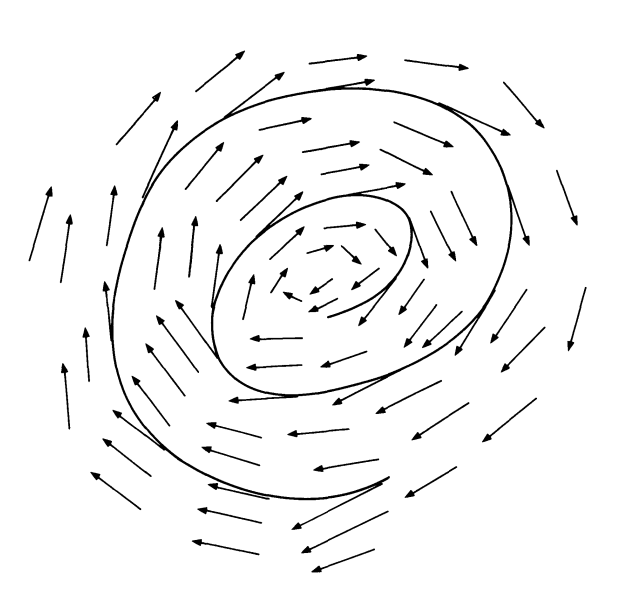
\includegraphics[scale=0.4]{fig2.5.PNG}
        \caption{An example of a vector field, $\mathbb{R}^3$}
        \label{fig:vectorfield}
    \end{center}
\end{figure}

A vector field in the context of the diagram is a function 
that will assign to every point a vector which points in the direction the spiral is moving:
from the outer part of the spiral to the inner part.

\newpage

\subsection{Geodesics}
Geodesics are curves on $\mathcal{M}^d$
which play the same role as straight
lines in $\mathbb{R}^d$, Euclidean space. 
An example of a geodesic on a sphere in $\mathbb{R}^3$ 
is given by the red curve on the sphere in the figure below, 
obtained from here \footnote{\url{https://en.wikipedia.org/wiki/Great-circle_distance
\#/media/File:Illustration_of_great-circle_distance.svg}}.
\begin{figure}[ht]
    \begin{center}
        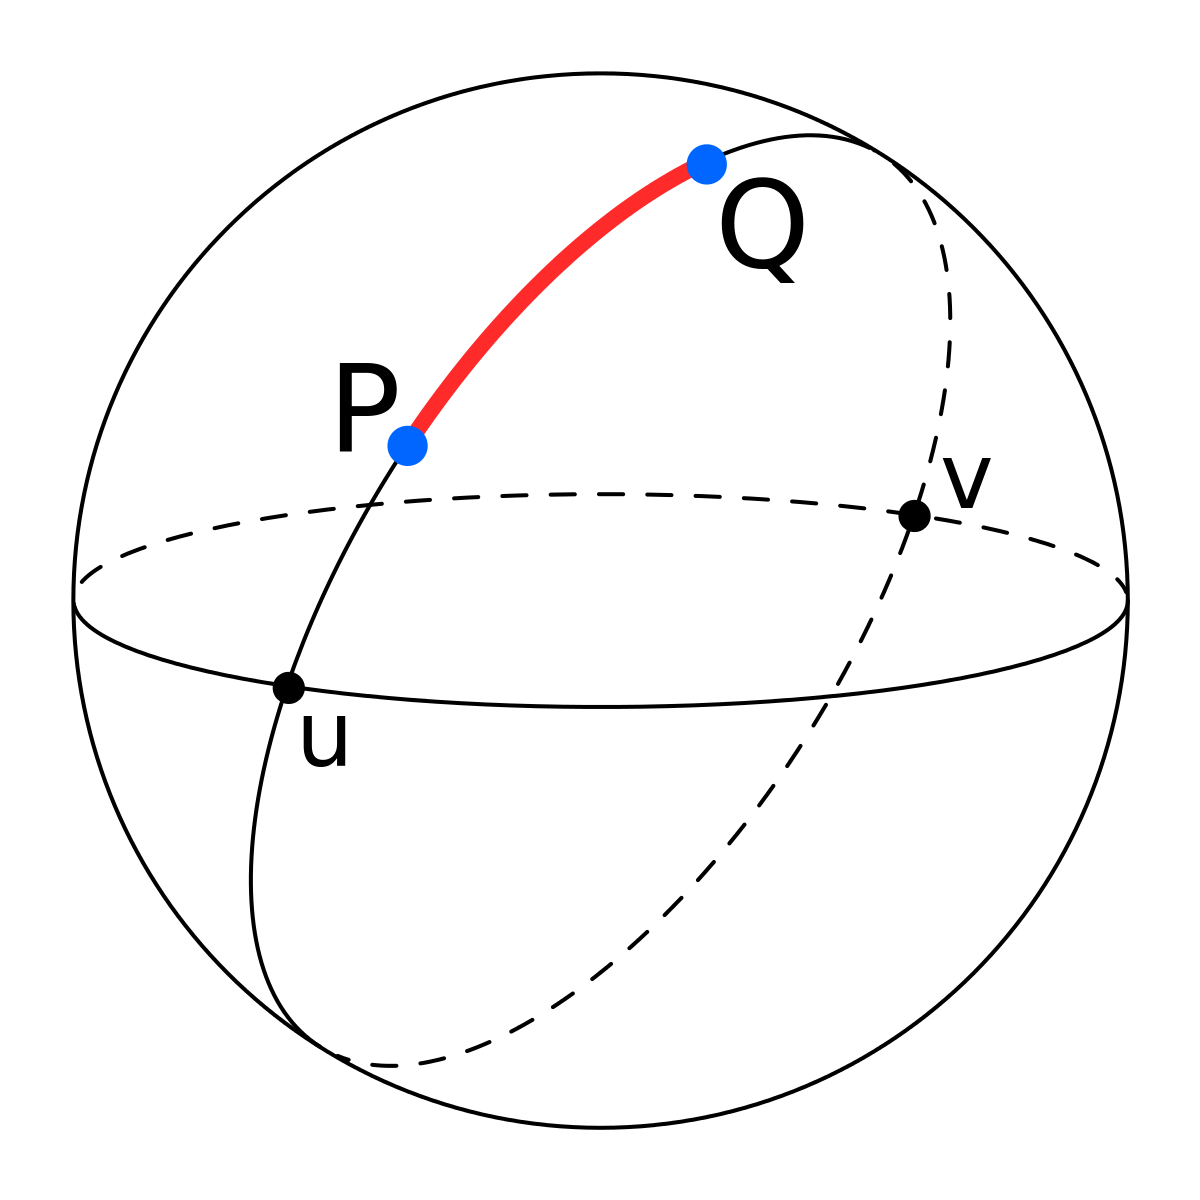
\includegraphics[scale=0.1]{geodesic.png}
        \caption{Geodesic between $P$ and $Q$ in red on a sphere in 
        $\mathbb{R}^3$}
        \label{fig:Illustration of a Geodesic}
    \end{center}
\end{figure}
\\
Then, for two points $p, q$,
while our usual Euclidean distance refers to $\norm{p-q}$, 
geodesic distance on the sphere in $\mathbb{R}^3$ 
is given by the arc length connecting the two points. Intuitively, 
geodesic distance can be thought of as the ``shortest path"
between two points on the manifold, $\mathcal{M}^d$.

\subsection{Exponential Maps}

The diagrams below were obtained from \footnote{\url{https://www.researchgate.net
/figure/An-exponential-map-exp-X-TX-M-M_fig1_224150233}}.\\
\textbf{Exponential Map:} For each $p \in \mathcal{M}^d$, let
$$exp_p(\mathbf{v}): T_p\mathcal{M} \longrightarrow \mathcal{M}^d$$
be the exponential map. 
\begin{figure}[ht]
    \begin{center}
        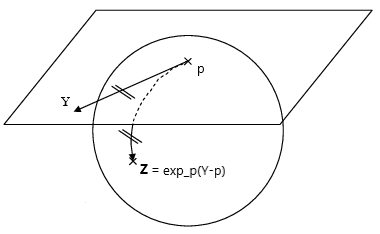
\includegraphics[scale=0.8]{exp_map.PNG}
        \caption{Illustration of the exponential map 
        for the three dimensional sphere}
        \label{fig:Illustration of an Exponential Map}
    \end{center}
\end{figure}
Let v be a vector $\mathbf{v} = Y - p$ for some $Y \in T_p\mathcal{M}$ we
wish to project onto $\mathcal{M}^d$. Then the exponential map moves along
the geodesic on $\mathcal{M}^d$ that mirrors the direction of $\mathbf{v}$
on $T_p\mathcal{M}$ and finds the projection of $Y$ on $\mathcal{M}^d$.\\
\\
\textbf{Logarithm Map:} For each $p \in \mathcal{M}^d$, let
$$log_p(z): \mathcal{M}^d \longrightarrow T_p\mathcal{M}$$
be the logarithm map. 
It is the inverse of the exponential map: 
given some point $z \in \mathcal{M}^d$, it finds the 
vector on $T_p\mathcal{M}$ that mirrors the geodesic 
going from $p$ to $z$. This vector indicates the direction in which $p$
should move to obtain the projection of 
$z \in \mathcal{M}^d$ onto $T_p\mathcal{M}$.
\begin{figure}[ht]
    \begin{center}
        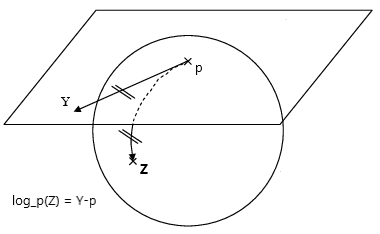
\includegraphics[scale=0.8]{log_map.PNG}
        \caption{Illustration of the log map 
        for the three dimensional sphere}
        \label{fig:Illustration of an log Map}
    \end{center}
\end{figure}

\newpage

\subsection{Tangent Space}
To define the tangent space we refer to the diagrams below.\\
Diagrams in figure 1.4 were obtained from here
\footnote{\url{https://en.wikipedia.org/wiki/Tangent_space\#/media/File:Image_Tangent-plane.svg}}
and here
\footnote{\url{https://www.researchgate.net/figure/
Conceptual-illustration-of-the-tangent-space-at
-point-P-on-a-Riemannian-manifold-M_fig2_262974373}}.

\begin{figure}[ht]
    \begin{center}
        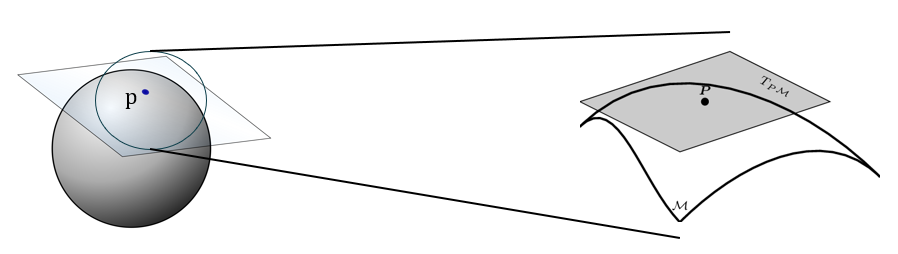
\includegraphics[scale=0.85]{tan_space_final.PNG}
        \caption{Illustration of the tangent space for the three 
        dimensional sphere}
        \label{fig:Illustration of Tangent Space}
    \end{center}
\end{figure}
\iffalse
\begin{figure}[ht]
\centering
\begin{subfigure}{.5\textwidth}
    \centering
    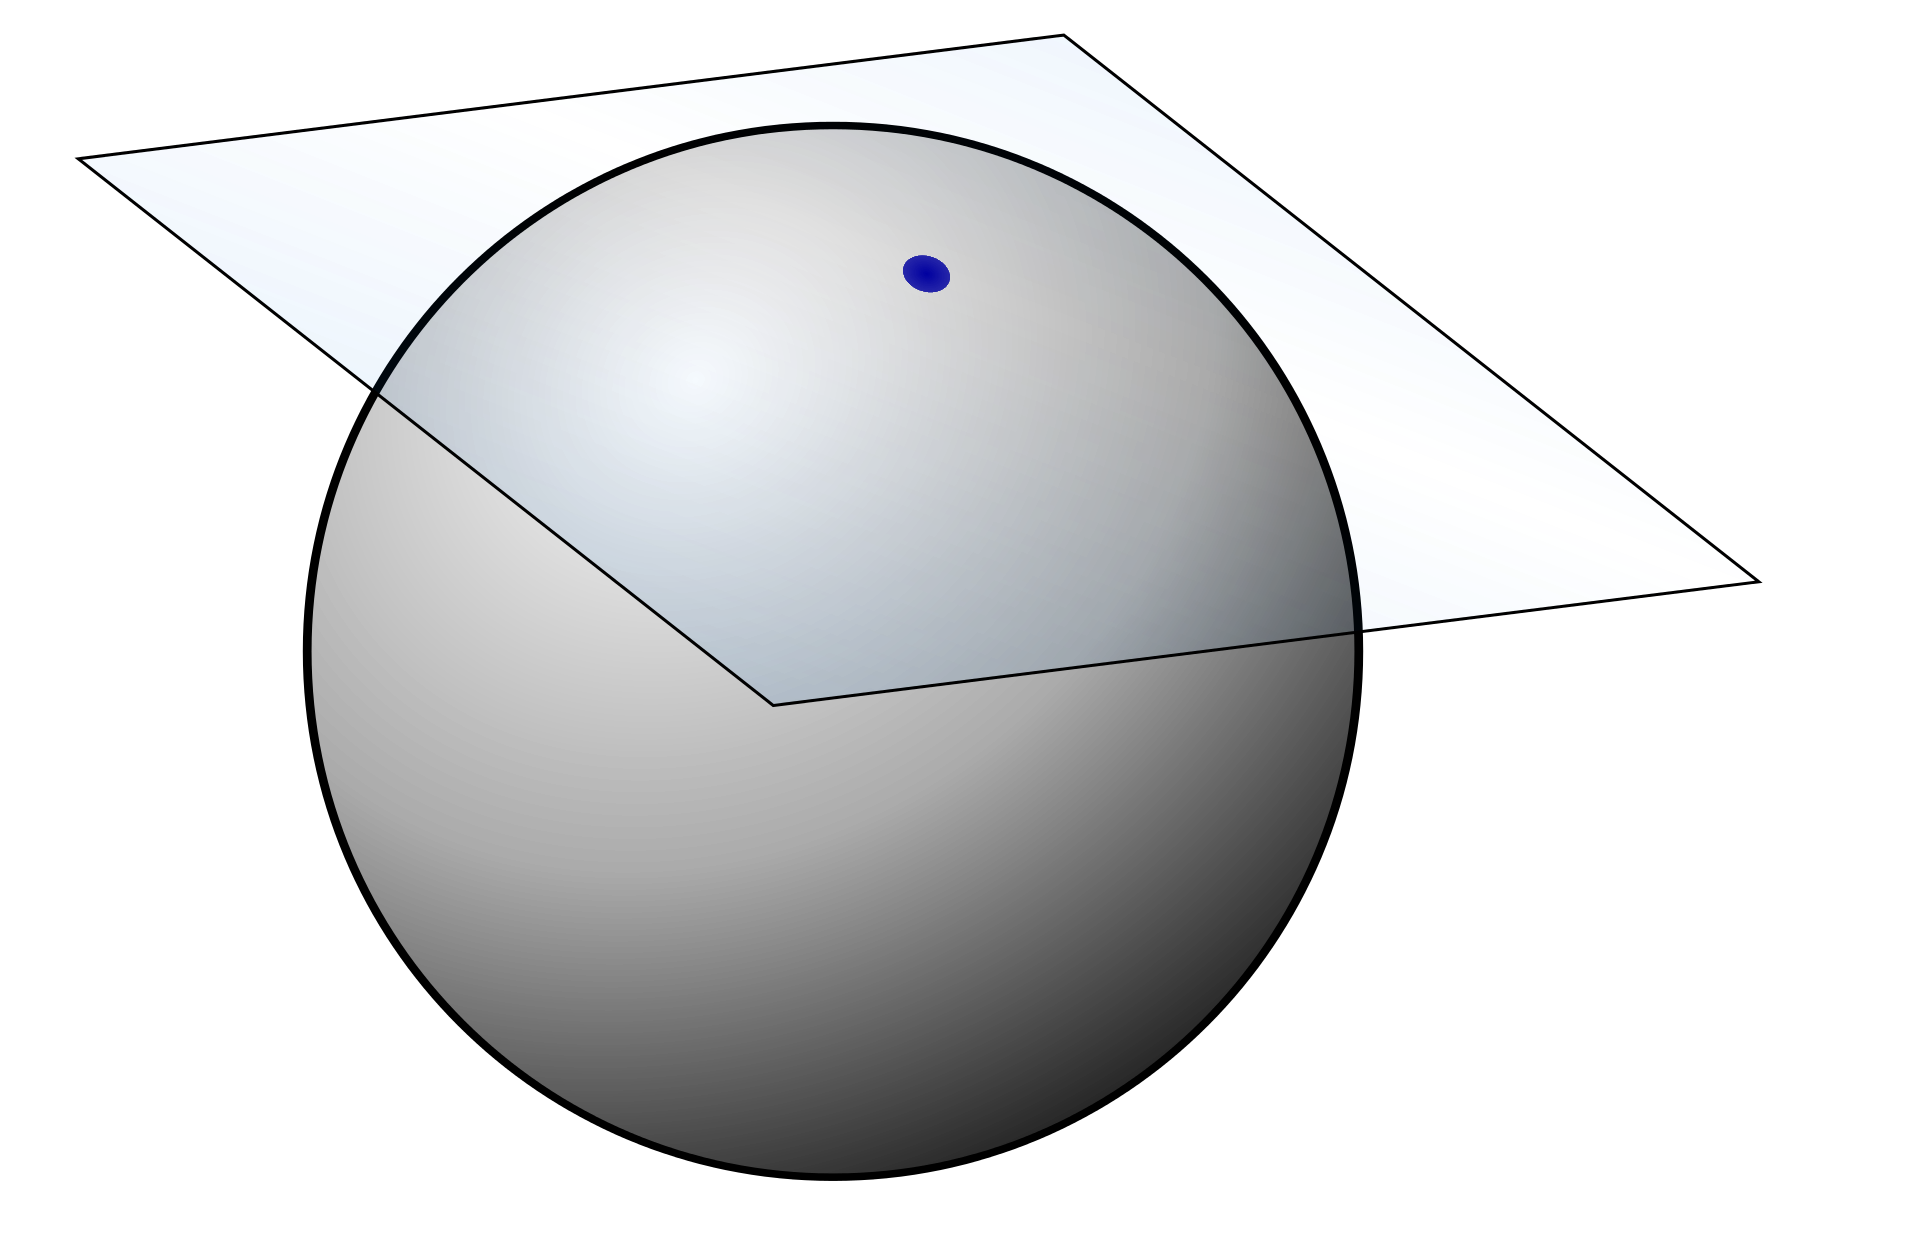
\includegraphics[scale=0.1]{tangent_space.png}
    \caption{Tangent Space of a Sphere}
    \label{tanspacesphere}
\end{subfigure}%
\begin{subfigure}{.5\textwidth}
    \centering
    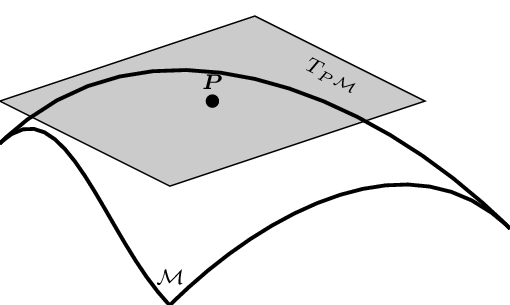
\includegraphics[scale=0.35]{tangent_space2.png}
    \caption{Close-up of the Tangent space in (a)}
    \label{tanspacemanifold}
\end{subfigure}
\caption{Illustration of a Tangent Space}
\label{fig:tanspaces}
\end{figure}
\fi
Let the three dimensional sphere be the manifold,
$\mathcal{M}^d$ and let the blue point be $p$.
Then the plane tangent to $\mathcal{M}^d$ at $p$ 
is the tangent space, $T_p\mathcal{M}$. Any vectors on
this plane lie in $T_p\mathcal{M}$. Then $exp_p$ would 
project points from the plane down onto the sphere, 
while $log_p$ would project points from the sphere 
up to the plane. This is the intuition of the tangent space
which we will be working with throughout this thesis.
Note that although we specify the 
manifold and tangent space in three dimensions, 
we can generalise this to $d$ dimensions, with $\mathcal{M}^d$
as the hypersphere in $d$ dimensions, while $T_p\mathcal{M}$ 
is the hyperplane. These are the definitions of $\mathcal{M}^d$
and $T_p\mathcal{M}$ we will use 
when we talk about principal flows later on in chapter three.

\newpage
 
\subsection{Eigenvalues and Eigenvectors}
Let $\mathbf{C} \in \mathbb{R}^{D \times D}$. 
Then a non-zero vector $\mathbf{v}$ is an eigenvector of $\mathbf{C}$ 
if there exists some scalar $\lambda$ such that $\mathbf{C}\mathbf{v} = \lambda \mathbf{v}$. 
Then $\lambda$ is known as the eigenvalue corresponding to vector $\mathbf{v}$.
Here we also note that for any two eigenvectors $v_i$ and $v_j$, $i \neq j$, $v_i \cdot v_j = 0$, 
or any two eigenvectors are orthogonal to each other, and that $v_i \cdot v_i = 1$.

\subsection{Diagonalisation}
We say that a matrix, $\mathbf{C}$, is diagonalisable if there exists 
an orthonormal matrix such that the rows of that orthonormal matrix 
are the eigenvectors of $\mathbf{C}$, and a diagonal matrix 
$\mathbf{\Lambda}$ whose diagonal entries are the eigenvalues of $\mathbf{C}$.
In the context of this report, we only consider 
the eigendiagonalisation of some covariance matrix 
$\mathbf{C} \in \mathbb{R}^{D \times D}$,
which is symmetric and thus, always diagonalisable. Formally,
the eigendiagonalisation of $\mathbf{C}$ is given by:
$$\mathbf{C} = \mathbf{V}\mathbf{\Lambda}\mathbf{V}^T$$
From here onwards, we assume there exists a function $diagonalise$ that
will perform eigendiagonalisation of a matrix and return us 
all eigenvectors and eigenvalues. We assume further that these
eigenvectors and eigenvalues are in sorted order, where 
the first eigenvector corresponds to the largest eigenvalue.

\chapter{Literature Review}

\section{Linear Dimension Reduction}

\subsection{Principal Component Analysis}

\iffalse
Note that centering each variable is the same as finding the "mean" 
observation $\bar{x} = \frac{1}{n}\sum^n_{i=1}x_i$, 
and subtracting that from every observation: $x_i - \bar{x}$, 
since $\bar{x}_i$ is the mean of the i-th variable.
This is done by calculating the covariance matrix 
of the centered data, $\mathbf{C}$, then 
computing the eigendiagonalisation of $\mathbf{C}$ 
and compute the dot product of the original 
data matrix by the $d$ eigenvectors associated with the 
$d$ largest eigenvalues.
\fi
\textbf{Principal Component Analysis (PCA)} introduced
here \cite{pca} and expanded in detail here \cite{pca2} tries to obtain a 
lower-dimensional representation of the data 
that retains as much variation as possible present in the data set. 
PCA relies on constructing principal components (PCs): 
new variables that are linear combinations of the original variables 
that have first been centered.
These PCs are uncorrelated (orthogonal) and ordered in descending order 
by the amount of variability of the original data retained.
Thus, PCA reduces some high-dimensional data of dimension $D$ 
to $d$ by computing the first $d$ PCs.\\
\begin{figure}[ht]
    \begin{center}
        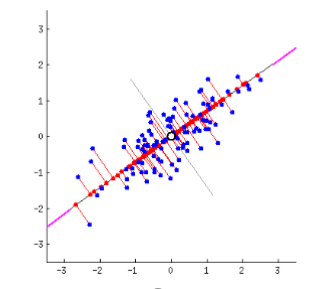
\includegraphics[scale=0.85]{pca_illust.PNG}
        \caption{PCA in 2 dimensions: data in blue, 
        principal direction as the black line, red points as the first 
        and only PC}
        \label{fig:PCA Illustration}
    \end{center}
\end{figure}
We construct these PCs by first centering the data matrix, $\mathbf{X}$, and
obtaining $\mathbf{X}_c$. Next we compute the covariance matrix of 
the centered data matrix: $\mathbf{C}$.
Then we compute the eigendiagonalisation of $\mathbf{C}$,
and obtain $\mathbf{V}_d$, a $D \times d$ matrix 
containing the $d$ eigenvectors associated 
with the $d$ largest eigenvalues. Here, we note that these $d$ eigenvectors
are the $d$ principal directions: directions onto which data is projected to
obtain the $d$ PCs. Principal directions will be mentioned
again in the later section on Principal Geodesic Analysis and in 
chapter three.
Finally, we get the $d$ PCs by computing $\mathbf{X}\mathbf{V}_d$.
\\
The PCA algorithm is outlined below. We assume for simplicity that the 
following functions are available:
$center$ that centers a given matrix and $covariance$ that computes the covariance
of a given matrix.
\begin{algorithm}
\KwResult{$\mathbf{X}_{(d)}$, the $d$ dimensional representation of $\mathbf{X}$, which are the $d$ PCs}
    $\mathbf{X}_c = center(\mathbf{X})$\;
    $\mathbf{C} = covariance(\mathbf{X}_c)$\;
    $\{v_1,...v_D\}, \{\lambda_1,...\lambda_D\} = diagonalise(\mathbf{C})$\;
    $\mathbf{V}_d = \{v_1,...v_d\}$\;
    $\mathbf{X}_{(d)} = \mathbf{X}\mathbf{V}_{d}$\;
    \Return{$\mathbf{X}_{(d)}$}
    \caption{PCA($\mathbf{X}$, $d$)}
\end{algorithm}

\subsection{Classical MDS, Euclidean Distance}
\textbf{Multidimensional Scaling (MDS)}'s 
main aim is find some $d$ dimensional representation of the
original data, $\mathbf{X}_{(d)}$,
that minimises the discrepancy between the pairwise distances 
of $\mathbf{X}$ and $\mathbf{X}_{(d)}$, 
given the squared matrix of pairwise distances of $\mathbf{X}$, $\mathbf{S}$.\\
Since dissimilarities do not change under translations, 
we can assume that $\mathbf{X}$ has column means equal to 0. 
Let $\mathbf{B} = \mathbf{X}\mathbf{X}^T$ be the gram matrix.
Let $\mathbf{J}$ be the centering matrix: 
$\mathbf{J} = \mathbf{I} - n^{-1}\mathbf{1}\mathbf{1}^T$, where 
$\mathbf{I} \in \mathbb{R}^{n \times n}$ and $\mathbf{1} \in \mathbb{R}^{n \times 1}$
Then, we run MDS by first computing  
$\mathbf{B} = -\frac{1}{2}\mathbf{J}\mathbf{S}\mathbf{J}$.
Next we compute the eigendiagonalisation of $\mathbf{B}$: 
$\mathbf{B} = \mathbf{V}\mathbf{\Lambda}\mathbf{V}^T$. 
From the original $\mathbf{V}$ we take the first $d$ columns: $\mathbf{V}_d$
and the first $d \times d$ submatrix of $\mathbf{\Lambda}$: $\mathbf{\Lambda}^{1/2}_d$.
Finally, we compute
$\mathbf{X}_{(d)} = \mathbf{V}_d\mathbf{\Lambda}^{1/2}_d$ to 
obtain the $d$-dimensional representation of the original data, $\mathbf{X}$. 
The MDS algorithm is outlined below. Assume we have a function $diagonalise$ which
computes the first $d$ columns of $\mathbf{V}$ and 
the $d \times d$ submatrix of $\mathbf{\Lambda}$.\\
\begin{algorithm}
\KwResult{$\mathbf{X}_{(d)}$, the $d$ dimensional representation of $\mathbf{X}$}
    $\mathbf{J} = \mathbf{I} - n^{-1}\mathbf{1}\mathbf{1}^T$\;
    $\mathbf{B} = -\frac{1}{2}\mathbf{J}\mathbf{S}\mathbf{J}$\;
    $\{v_1,...v_D\}, \{\lambda_1,...\lambda_D\} = diagonalise(\mathbf{B})$\;
    $\mathbf{V}_d, \mathbf{\Lambda}_d = \{v_1,...v_d\}, \{\lambda_1,...\lambda_d\}$\;
    $\mathbf{X}_{(d)} = \mathbf{V}_d\mathbf{\Lambda}^{1/2}_d$\;
    \Return{$\mathbf{X}_{(d)}$}
    \caption{MDS($\mathbf{S}$, $d$)}
\end{algorithm}
Note that using Euclidean distances, the result of MDS is the same as PCA. 
The algorithm and details above are taken from \cite{mds} and for a 
more detailed treatment of MDS we refer there as well. The plot below, obtained from
\footnote{\url{http://statweb.stanford.edu/~jtaylo/courses/stats306B/mds.html}} 
showcases the results of applying MDS to digits, and visualising the results in 
two dimensions. 
\begin{figure}[ht]
    \begin{center}
        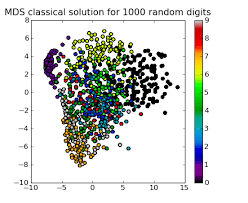
\includegraphics[scale=1]{mds_result.png}
        \caption{Results from Multidimensional Scaling}
        \label{fig:MDS results}
    \end{center}
\end{figure}

\newpage
\section{Non-Linear Dimension Reduction}

Non-linear dimensionality reduction methods are particularly useful 
when the multivariate data we obtain is sampled 
from a smooth non-linear manifold $\mathcal{M}^d$, 
e.g a manifold in an S-shape or a hypersphere.
This class of methods obtain better estimates than linear methods like PCA and MDS,
especially for the data mentioned above. 
They are especially successful as certain data sets contain 
essential non-linear structures that are invisible to PCA and MDS.

\newpage

\subsection{Isomap}

\textbf{Isomap}, introduced by Tenenbaum et al. \cite{isomap} is an extension 
of MDS to manifolds in which embeddings 
are optimized to preserve geodesic distances between pairs of data points.
Isomap achieves this by estimating the geodesic distance between data points, 
given only input-space distances, e.g Euclidean distance between points.
\\
This relies on the fact that for neighboring points, 
input-space distance provides a good approximation to geodesic distance. 
For faraway points, Isomap approximates geodesic distance 
by adding up a sequence of “short hops” between neighboring points, 
computed efficiently by finding shortest paths in a graph with edges 
connecting neighboring data points.\\
Tenenbaum et al. \cite{isomap} show this by proving that for a 
sufficiently high density of data points, 
we can always choose a neighborhood size large enough 
that the graph will (with high probability) have a path not much longer 
than the true geodesic, but small enough to prevent edges 
that ``short circuit” the true geometry of the manifold.
This is illustrated in the diagram below, obtained from \cite{isomap}.\\
\begin{figure}[ht]
    \begin{center}
        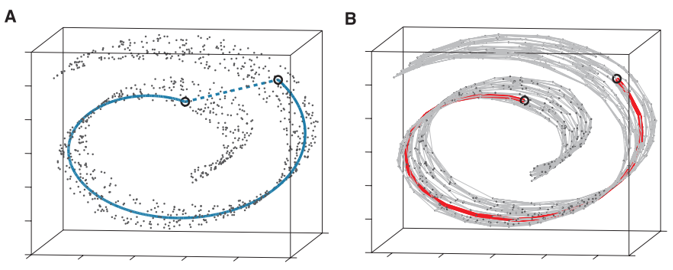
\includegraphics[scale=0.85]{isomap.PNG}
        \caption{Isomap: A the dotted-line distance ``short circuits" the manifold
        , The solid red path in B does not.}
        \label{fig:Isomap}
    \end{center}
\end{figure}
Like MDS, Isomap takes as input $\mathbf{S}$: 
a matrix of dissimilarities but differs by first 
constructing the neighbourhood graph, $G$. We start by creating nodes for every 
data point $i$. Given some user input $K$,
for every point $i$, Isomap adds an edge between
the $i$ and another point $j$ with weight $S_{i,j}$ if $j$ is 
one of $i$'s $K$ nearest neighbours. We then run an all pairs shortest path 
algorithm on $G$ (we use FloydWarshall here), and obtain a new matrix 
$\mathbf{A}$, where $\mathbf{A}_{i,j}$ is the shortest distance from $i$ to $j$. 
This approximates geodesic distance between $i$ and $j$. 
Then we run $MDS(\mathbf{A}, d)$ to obtain $\mathbf{X}_{(d)}$. \\
The algorithm is outlined below. For simplicity, 
assume we have a function $ConstructGraph$ which 
constructs the graph $G$ as explained above.
\begin{algorithm}
\KwResult{$\mathbf{X}_{(d)}$, the $d$ dimensional representation of $\mathbf{X}$}
    $G = ConstructGraph(\mathbf{S}, K)$\;
    $\mathbf{A} = FloydWarshall(G)$\;
    \Return{MDS($\mathbf{A}$, $d$)}
    \caption{Isomap($\mathbf{S}$, $d$, $K$)}
\end{algorithm}

\newpage

\subsection{Locally Linear Embeddding}

\textbf{Locally Linear Embedding (LLE)} introduced by 
Saul and Roweis \cite{lle} aims to construct 
a mapping from the $D$ dimensional 
original points to the $d$ dimensional reconstructed points
that preserves the local configurations of each point's nearest neighbors. 
Locally, LLE assumes the embedding is linear, 
and for each data point $p \in \mathbb{R}^D$, 
LLE uses a linear combination of its $K$ nearest neighbours 
to reconstruct a lower-dimensional $p_d \in \mathbb{R}^d$. \\
Let the set of the $i$-th point's $k$ nearest neighbours be $N^i_k$.
LLE starts by learning some weights from the $D$-dimensional data: 
$\mathbf{W}$ by minimizing the \textbf{Reconstruction Error} 
below using constrained linear fits.
$$\mathbf{RE}(\mathbf{W}) = \sum_i^n|\mathbf{X}_i - \sum_{j \in N^i_k}^K \mathbf{W}_{ij} \mathbf{X}_j|^2$$
Here, $\mathbf{W}$ are the weights that best reconstruct each 
data point from it's $K$ neighbours, and
$\mathbf{W}_{ij}$ represents the contribution 
of the j-th data point in reconstructing the i-th one.
These weights obey an important symmetry: for any particular data point,
they are invariant to rotations, rescalings, and translations
of that data point and its neighbors.
They thus reflect intrinsic geometric properties 
of the data that are invariant to such transformations,
and therefore, we expect their characterization of local geometry in the 
original data space to be equally valid for local patches on the manifold.
This is what motivates our use of $\mathbf{W}_{ij}$ in reconstructing
the embedded manifold coordinates in $d$ dimensions. \\
Next, compute the vectors $\mathbf{Y}_i$ best 
reconstructed by the weights $\mathbf{W}_{ij}$ 
by choosing the $d$ dimensional coordinates of each output
that minimise the \textbf{Embedding Cost Function}: 
$$\mathbf{EC}(\mathbf{Y}) = \sum_i |\mathbf{Y}_i - \sum_j \mathbf{W}_{ij}\mathbf{Y}_j|^2$$
At the end of LLE, each $D$-dimensional observation $\mathbf{X}_i$ 
is mapped to a $d$ dimensional $\mathbf{Y}_i$ 
representing global internal coordinates on the manifold.\\
A diagram loosely illustrating the procedure above, obtained from \cite{lle}, 
is shown below.
\begin{figure}[ht]
    \begin{center}
        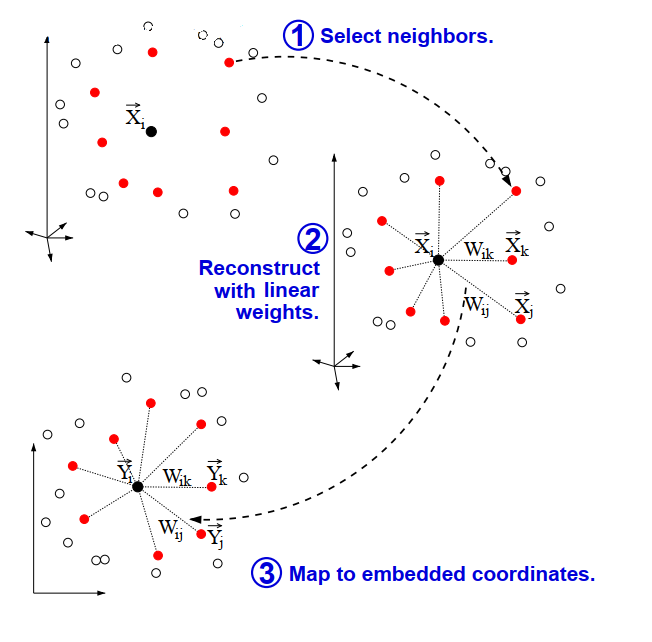
\includegraphics[scale=0.55]{LLE.png}
        \caption{Illustration of Locally Linear Embedding Procedure}
        \label{fig:Illustration of LLE Process}
    \end{center}
\end{figure}
\begin{algorithm}
\KwResult{$\mathbf{X}_{(d)}$, the $d$ dimensional representation of $\mathbf{X}$}
    First compute $N^i_k$ for all $x_i$\;
    $\mathbf{W} = argmin_{\mathbf{W}}\sum_i^n|x_i - \sum_{j \in N^i_k}^k \mathbf{W}_{ij} x_j|^2$\;
    $\mathbf{X}_{(d)} = argmin_{\mathbf{Y}}\sum_i |\mathbf{Y}_i - \sum_{j \in N^i_k}^k \mathbf{W}_{ij}\mathbf{Y}_j|^2$\;
    \Return{$\mathbf{X}_{(d)}$}
    \caption{LLE($\mathbf{X}$, $d$, $k$)}
\end{algorithm}

\subsection{Principal Geodesic Analysis}
\iffalse
by finding a sequence of lower-dimensional subspaces, 
which on manifolds are nested geodesic submanifolds 
that maximize the projected variance of the data. 
These submanifolds are called the principal geodesic submanifolds, 
which are analogous to linear subspaces in PCA.\\
Let $U \subset T_p\mathcal{M}$ be a neighbourhood of 0 in which our data, 
$\mathbf{X}$ lies, such that projection is well defined 
for all geodesic submanifolds of $exp_p(U)$.These principal geodesic submanifolds 
are obtained by first constructing an orthonormal basis of tangent vectors 
$v_1,...,v_d \in T_p\mathcal{M}$ that span the tangent space. 
These vectors are then used to form the principal geodesic subspaces 
$H_k$ where $H_k = exp_p(V_k)$, and $V_k$ is intersection of the 
subspace spanned by vectors $1..k$ and $U$.
subspace $V_k = span(\{v_1,...,v_k\})\bigcap U$.
\fi
\textbf{Principal Geodesic Analysis (PGA)} introduced here \cite{pga}, 
is a generalization of PCA to manifolds. 
The main aim of PGA is to describe some $D$ dimensional data that
lie on $\mathcal{M}^d$ embedded in $\mathbb{R}^D$.
Let $T_p\mathcal{M}$ be the tangent space of $\mathcal{M}^d$ 
at the intrinsic mean $p$ of the data. 
The intrinsic mean here is the extension of the concept 
of the mean in Euclidean space to manifolds.
PGA aims to construct some principal geodesics that are analogous
to principal directions in PCA: the directions along which data is
projected to obtain a PC.\\
Instead of finding the principal geodesic however, Fletcher et al. prove that
we can approximate the $d$ geodesics along which maximal variation lies 
by projecting data from $\mathcal{M}^d$ to $T_p\mathcal{M}$ where 
$p$ is the intrinsic mean of $\{x_1,..x_n\}$
and then finding the 
$d$ eigenvectors associated with the $d$ largest eigenvalues of the 
covariance matrix of the projected data.\\
PGA begins with computing $p$ by first setting 
$p$ to a random data point, 
then iteratively obtaining a better estimate of $p$. Let $p_i$ be the 
estimate of $p$ at the i-th iteration.
At the i-th iteration, we compute the average of the vectors obtained 
using the $log_{p_{i-1}}(x_i), \forall x_i$ then set $p_{i}$ 
as the projection of that average using $exp_{p_{i-1}}$.\\
After obtaining $p$, we calculate the vectors $u_i = log_p(x_i), \ \forall x_i$.
Next we calculate the covariance matrix 
$\mathbf{C} = \frac{1}{n} \sum^n_{i=1} u_iu_i^T$.
Finally we diagonalise $\mathbf{C}$ to obtain $\{v_k, \lambda_k\}$ 
the eigenvectors and eigenvalues respectively, 
which represent the principal directions 
in the tangent space $T_p\mathcal{M}$ and the variances.
\begin{figure}[ht]
    \begin{center}
        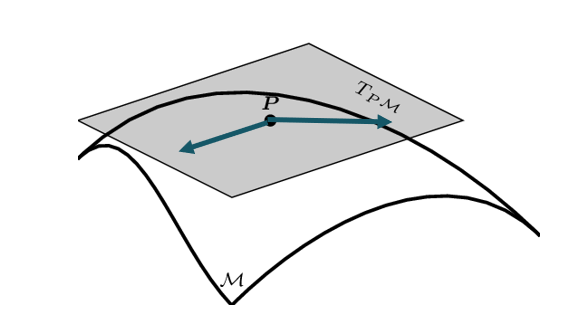
\includegraphics[scale=0.45]{pga_directions.PNG}
        \caption{An illustration of PGA directions 
        in tangent space approximating principal geodesics}
        \label{fig:Directions On Tangent Space}
    \end{center}
\end{figure}\\
The algorithm for PGA is outlined below.
\begin{algorithm}
\KwResult{$\{v_1,...v_D\} \in T_p\mathcal{M}$, principal directions and \\
Variances $\{\lambda_1,...\lambda_D\} \in \mathbb{R}$}
    $p = $ intrinsic mean of data $\{x_1,....x_n\}$\;
    $u_i = log_p(x_i)$\;
    $\mathbf{C} = \frac{1}{N}\sum^N_{i=1}u_i u_i^T$\;
    $\{v_1,...v_D\}, \{\lambda_1,...\lambda_D\} = diagonalise(\mathbf{C})$\;
    \Return{$\{v_1,...v_D\}, \{\lambda_1,...\lambda_D\}$}
    \caption{PGA($\{x_1,...x_n\}$)}
\end{algorithm}

\chapter{Greedy Principal Flows}

\section{Goal Of Research}
The main objective for greedy principal flows is to quantify or describe 
multivariate data on the manifold: we cannot simply fit a line, 
as this is not Euclidean space.
Instead, we want some curve or path such that,
locally, it follows the path of maximal variation of the data in some neighbourhood, 
but globally also provides the path of maximal ``cumulative" variation of the data.
These motivate our definition of the principal flow:
it is a curve or path on the manifold passing 
through the mean of the data 
that is always tangent to the direction of maximal variation 
of the data at any given point it contains. 
This path flows outward from the center of the principal flow, 
the centroid of the data as in the diagram below.
The vectors tangent to every point of the principal flow forms a vector field,
illustrated by the arrows on the red curve,
and each points in the direction of maximum variance.
\begin{figure}[ht]
    \begin{center}
        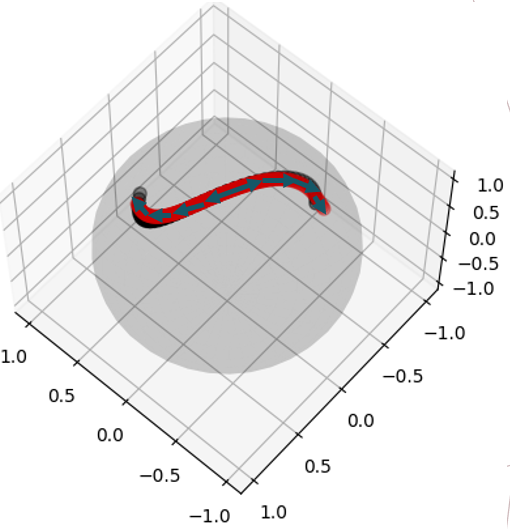
\includegraphics[scale=0.85]{flow_vector_field.PNG}
        \caption{The principal flow as a vector field, with the flow in red.}
        \label{fig:Vector Field Principal Flow}
    \end{center}
\end{figure}
The problem of constructing principal flows 
has already been solved in \cite{principalflow}, 
where they were constructed by 
solving a problem in variational calculus. \\
Therefore, we focus instead on constructing the principal flow using a novel, 
simpler to implement approach: a greedy algorithm. 
Here we note that we focus on 
the first order principal flow, which can be thought of as 
the manifold extension of the first principal direction in Euclidean space.
Additionally, we simplify our approach further and 
assume that our data $\mathbf{X}$ is some $D$ dimensional
data lying on a hypersphere $\mathcal{M}^d$.
Thus, our goal is to implement this greedy, simpler version of the
principal flow algorithm, 
and experiment with the results that this implementation of the
principal flow algorithm brings. 
How would it describe various, popular multivariate
datasets? Could it find novel ways of describing popular,
existing high-dimensional data?

\section{Centroid Algorithm}
Before we get into our principal flow algorithm, we first need to 
establish our starting point. Since our principal flow 
follows the path of maximal variation of our data, 
we know it should pass through the centroid of the data. 
However, since the data lies on a manifold, we cannot simply use the 
Euclidean mean of the data points. We need to find the centroid of the data
lying on the manifold.
Thus, we first aim to estimate this centroid and use it as a starting point.
Although there are many ways of doing this,
including the method to find the intrinsic mean in chapter 2.2.3,
we opt to make use of the fact that 
the first principal direction passes through the centroid of the data.
To see why this is so, we start with the idea that the first principal direction
is the direction that maximises the variance of the data. 
This can be shown to be equivalent to minimising the reconstruction error of 
the points projected on this principal direction, 
which is minimising the sum of squared residuals
$\sum(x_i - \hat{x}_i)^2$ where $\hat{x}_i$ are the projected points and 
$x_i$ are our data points. 
Notice that this is minimised by obtaining $\hat{x}_i$
that lie on the ordinary least squares (OLS) regression line.
And since we can prove that the mean of the data or the centroid of the data
lies on the OLS regression line, the centroid of the data 
does indeed lie on the first principal direction.
Thus, if we iteratively project all the data onto the tangent space of the hypersphere, 
find the first principal direction, move in that direction, 
and find the projected point on the hypersphere, we will eventually converge on the 
centroid. The algorithm to find the centroid is outlined below.
\begin{algorithm}
\KwResult{$p$, centroid of the data}
    $p = $ a random data point from $\{x_1,....x_n\}$\;
    \For{$i = 1 \to max\_iter$}{
        Compute $u_i = log_p(x_i)$ for all $x_i$,\;
        $\mathbf{C} = \frac{1}{N}\sum^N_{i=1}u_i u_i^T$\;
        $v_1 = $ eigenvector corresponding to the largest eigenvalue of $\mathbf{C}$\;
        $p' = p + \epsilon v_1$\;
        $p = exp_p(p')$\;
    }
    \Return{$p$}
    \caption{Centroid($\{x_1,...x_n\}$)}
\end{algorithm}

\iffalse
\textbf{Problem}:
With our starting point settled, we observe that the principal flow algorithm may run
into a problem: What if our data stretches all around the hypersphere? 
How do we deal with projecting
data through the sphere?\\
To solve this, instead of taking all data into consideration, 
we use a kernel function, $\mathcal{K}$ to choose a small neighborhood around
our current principal flow point, whose size is controlled by $h$. 
For our algorithm, we implement 2 choices of kernel functions: The binary kernel 
includes points in some neighbourhood and excludes points outside,
while the gaussian kernel weights points according to 
the gaussian distribution based on their distance from the original point.\\
Thus, we project the data within some neighbourhood $\mathbf{X}$ onto the tangent space 
at the centroid, p: $T_p\mathcal{M}$. We use the logarithm map, $log_p$ to do this. 
Then the path of maximal variation in this neighbourhood of points 
is the first principal direction of this data from PCA. This direction 
is obtained by diagonalising the covariance matrix of the data on this tangent
space. \\
\textbf{Problem}:
This direction clearly is not accurate if we only move in this direction,
since it will eventually lead us out of the surface of the hypersphere, and even on the 
hypersphere, the neighbourhood of points may differ, and change the direction 
of the path of maximal variation.\\
Thus, instead of only using this direction, we move infinitesimally in this first direction,
then carry out the same procedure again. Thus we iteratively find the "local"
direction of maximal variation, move in that direction, and re-compute the next direction
of maximal variation. We continue doing this until we have obtained a flow through the
entire data set.\\
This does indeed follow the framework that isomap and LLE abide by
as well: that obtaining the best option locally becomes the best option globally as well. 
This is exactly the idea of this Greedy Principal flow algorithm. 
\fi
\section{Algorithm}

Now we move on to outlining and elaborating on the greedy principal flow algorithm.
Let $p_i$ be the point on the principal flow
obtained from the i-th iteration where $p_0$ is the 
first point on the principal flow: the centroid from the 
algorithm in the previous section. Before we start our principal flow
algorithm we first need to decide on the maximum number of iterations. 
This will determine the number of points on each side of the principal flow, 
not counting the original point: the centroid.
Now we explain the procedure of the principal flow at the $i$-th iteration.\\
We note that for the $i$-th iteration, we apply the following procedure
to both ends of the principal flow.
First, we project $\mathbf{X}$ onto the hyperplane
at $p_{i-1}$, $T_{p_{i-1}}\mathcal{M}$.
\iffalse
However, we realise we may run into a problem: 
What if our data stretches all around the hypersphere? 
How do we deal with projecting data through the sphere?\\
To solve this, instead of projecting all data, 
we use a kernel function, $\mathcal{K}$ to choose a small neighborhood around
our current principal flow point, whose size is controlled by scale parameter $h$. 
\fi
Here we may choose to project all our data, or use a kernel function, 
$\mathcal{K}$ to weight our data so that more emphasis is 
placed on points in some neighborhood around
$p_{i-1}$, whose size is controlled by scale parameter $h$, than outside it.
Intuitively, $h$ controls how sensitive the principal flow is to local data.
We define $\{w_i,....w_n\}$ as the weights from our kernel function.
For our algorithm, we implement three choices of kernel functions: the binary kernel 
which weights points as one or zero depending on their distance from 
$p$, the gaussian kernel which weights points according to 
the gaussian distribution based on their distance from $p$ and
lastly the identity kernel, which sets all weights to be one.\\
Thus, we first apply our kernel function to the data, and obtain weights 
$\{w_i,....w_n\}$, then apply our log map $log_{p_{i-1}}$ to project our data on 
$T_{p_{i-1}}\mathcal{M}$ obtaining a matrix of vectors on 
$T_{p_{i-1}}\mathcal{M}$ that point from $p$
to the projected points. These $log_{p_{i-1}}(x_i)$ are our plane vectors.
Then we compute the covariance matrix of the plane vectors
using both our weights and our plane vectors
by the equation below obtained from \cite{principalflow}.
$$C_h(p) = \frac{1}{\Sigma_i \mathcal{K}_h(x_i,p)}\sum^n_{i=1}(log_{p_{i-1}}(x_i)\otimes log_{p_{i-1}}(x_i))\mathcal{K}_h(x_i,p)$$
We then perform eigendiagonalisation of the covariance matrix and 
take the eigenvector $v_1$ corresponding to the largest eigenvalue $\lambda_1$. 
This indicates the direction of the principle flow 
and is our principal direction. Here, $\lambda_1$ corresponds to the amount
of variance of our data in the direction of $v_1$.
This is where the ``greediness'' in 
our algorithm lies: since we choose at each step, the direction of maximum 
variance.\\
If this is the first iteration, then $p_{i-1}$ is the centroid of the data.
Thus, we collect two points: 
one point when we move a step size of $\epsilon$ in the principal direction, 
and the other when we move a step size of $\epsilon$ in the 
opposite of the principal direction. We then project both points back onto 
$\mathcal{M}^d$, using $exp_{p_{i-1}}$. 
Set $p_1$ to be the first point, and $p\_opp_1$ to be the second. 
Otherwise, we first check that this principal direction is in the same 
direction as the previous principal direction of this end of the flow, 
and if not, apply a negative sign to the principal direction. 
Then for each end of the flow,
we move a step size of $\epsilon$ in the principal direction
at that end, then project both points back onto 
$\mathcal{M}^d$, using the exponential map.\\
We repeat the procedure above until the maximum iterations is reached.
\newpage
\begin{figure}[ht]
    \begin{center}
        \includegraphics[scale=0.055]{main_flow_procedure.png}
        \caption{Illustration of the Greedy Princpal flow algorithm. 
        The first four steps cover the first iteration, while five and 
        six cover the i-th iterations.}
        \label{fig:Greedy Principal Flow Procedure}
    \end{center}
\end{figure}

The Greedy Principal Flow algorithm is outlined below.
\begin{algorithm}
\KwResult{$\{p_0,..,p_{m}\} \bigcup \{p\_opp_1,..,p\_opp_{m}\}$, points on the principal flow}
    $m = max\_iter$\;
    $p_0 = centroid$\;
    $p\_opp_0 = centroid$\;
    \For{$i = 1 \to m$}{
        \If{$i == 1$}{
            $\{w_i,....w_n\} = \mathcal{K}(h, p_{i-1}, \{x_1,....,x_n\})$\;
            $\mathbf{C}_h(p_{i-1}) = \frac{1}{\Sigma_i w_i}\sum^n_{i=1}(log_{p_{i-1}}(x_i)\otimes log_{p_{i-1}}(x_i))w_i$\;
            $\{v_1,...,v_n\}, \{\lambda_1,...\lambda_n\} = diagonalise(\mathbf{C}_h(p_{i-1}))$\;
            $principal\_direction = v_1$\;
            $principal\_direction\_opp = -v_1$\;
        }
        \Else{
            $\{w_i,....w_n\} = \mathcal{K}(h, p_{i-1}, \{x_1,....,x_n\})$\;
            $\mathbf{C}_h(p_{i-1}) = \frac{1}{\Sigma_i w_i}\sum^n_{i=1}(log_{p_{i-1}}(x_i)\otimes log_{p_{i-1}}(x_i))w_i$\;
            $\{v_1,...,v_n\}, \{\lambda_1,...\lambda_n\} = diagonalise(\mathbf{C}_h(p_{i-1}))$\;
            \If{$cos^{-1}(v_1^Tprincipal\_direction\_past) > \pi/2$}{
                $v_1 = -v_1$\;
            }
            $principal\_direction = v_1$\;
            $\{w_i,....w_n\} = \mathcal{K}(h, p\_opp_{i-1}, \{x_1,....,x_n\})$\;
            $\mathbf{C}_h(p\_opp_{i-1}) = \frac{1}{\Sigma_i w_i}\sum^n_{i=1}(log_{p\_opp_{i-1}}(x_i)\otimes log_{p\_opp_{i-1}}(x_i))w_i$\;
            $\{v_1,...,v_n\}, \{\lambda_1,...\lambda_n\} = diagonalise(\mathbf{C}_h(p\_opp_{i-1}))$\;
            \If{$cos^{-1}(v_1^Tprincipal\_direction\_opp\_past) > \pi/2$}{
                $v_1 = -v_1$\;
            }
            $principal\_direction\_opp = v_1$\;
        }
        $p_i = exp_{p_{i-1}}(p_{i-1} + \epsilon principal\_direction)$\;
        $p\_opp_i = exp_{p\_opp_{i-1}}(p\_opp_{i-1} + \epsilon principal\_direction\_opp)$\;
        $principal\_direction\_past = principal\_direction$\;
        $principal\_direction\_opp\_past = principal\_direction\_opp$\;
    }
    \Return{$\{p_0,..,p_{m}\} \bigcup \{p\_opp_1,..,p\_opp_{m}\}$}
    \caption{GreedyPrincipalFlow($\{x_1,...x_n\}$, $centroid$, $\mathcal{K}$, $max\_iter$, $h, \epsilon$)}
\end{algorithm}

\newpage 
\section{Extension: Greedy Principal Boundary}

\begin{figure}[ht]
    \begin{center}
        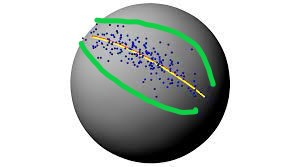
\includegraphics[scale=1.2]{boundary_on_sphere.png}
        \caption{Principal Boundary in green around the data in blue
        for the three dimensional sphere}
        \label{fig:Principal Boundary}
    \end{center}
\end{figure}

In the section above, we have already seen the principal flow.
Now we extend the idea of principal flows to attempt to find some boundary of the data.
Let us assume that the data is contained on some ellipse of the manifold
$\mathcal{M}^d$. Then our aim is to find some boundary around this ellipse. We proceed 
similarly to the principal flow, except that 
we now save $v_1, v_2, \lambda_1, \lambda_2$
when we diagonalise $\mathbf{C}_{h}(p_{i-1})$.
and use them to compute the boundaries of data.\\
Let $b_{i,1}$ be the first boundary point of the i-th
principal flow point.
Then at each iteration, the boundary $b$ is calculated before $p$ 
is updated by $b_{i,1} = exp_{p_{i-1}}(p_{i-1} + \frac{\lambda_2}{\lambda_1}*radius*v_2)$ and
$b_{i,2} = exp_{p_{i-1}}(p_{i-1} - \frac{\lambda_2}{\lambda_1}*radius*v_2)$
where radius is a user specified parameter. Intuitively, 
we try to move a distance in the direction of $v_2$ orthogonal to the principal flow
that approximates the radius of the ellipse that contains the data, $\mathbf{X}$.
\begin{algorithm}
\KwResult{$\{p_0,..,p_{m}\} \bigcup \{p\_opp_1,..,p\_opp_{m}\} \bigcup \{b_{0,1},..,b_{m-1,2}\} \bigcup \{b\_opp_{1,1},..,b\_opp_{m-1,2}\}$, points and boundary of the principal flow}
    $m = max\_iter$\;
    $p_0 = centroid$\;
    $p\_opp_0 = centroid$\;
    \For{$i = 1 \to m$}{
        \If{$i == 1$}{
            $\{w_i,....w_n\} = \mathcal{K}(h, p_{i-1}, \{x_1,....,x_n\})$\;
            $\mathbf{C}_h(p_{i-1}) = \frac{1}{\Sigma_i w_i}\sum^n_{i=1}(log_{p_{i-1}}(x_i)\otimes log_{p_{i-1}}(x_i))w_i$\;
            $\{v_1,...,v_n\}, \{\lambda_1,...\lambda_n\} = diagonalise(\mathbf{C}_h(p_{i-1}))$\;
            $b_{i-1,1} = exp_{p_{i-1}}(p_{i-1} + \frac{\lambda_2}{\lambda_1}*radius*v_2)$\;
            $b_{i-1,2} = exp_{p_{i-1}}(p_{i-1} - \frac{\lambda_2}{\lambda_1}*radius*v_2)$\;
            $principal\_direction = v_1$\;
            $principal\_direction\_opp = -v_1$\;
        }
        \Else{
            $\{w_i,....w_n\} = \mathcal{K}(h, p_{i-1}, \{x_1,....,x_n\})$\;
            $\mathbf{C}_h(p_{i-1}) = \frac{1}{\Sigma_i w_i}\sum^n_{i=1}(log_{p_{i-1}}(x_i)\otimes log_{p_{i-1}}(x_i))w_i$\;
            $\{v_1,...,v_n\}, \{\lambda_1,...\lambda_n\} = diagonalise(\mathbf{C}_h(p_{i-1}))$\;
            $b_{i-1,1} = exp_{p_{i-1}}(p_{i-1} + \frac{\lambda_2}{\lambda_1}*radius*v_2)$\;
            $b_{i-1,2} = exp_{p_{i-1}}(p_{i-1} - \frac{\lambda_2}{\lambda_1}*radius*v_2)$\;
            \If{$cos^{-1}(v_1^Tprincipal\_direction\_past) > \pi/2$}{
                $v_1 = -v_1$\;
            }
            $principal\_direction = v_1$\;
            $\{w_i,....w_n\} = \mathcal{K}(h, p\_opp_{i-1}, \{x_1,....,x_n\})$\;
            $\mathbf{C}_h(p\_opp_{i-1}) = \frac{1}{\Sigma_i w_i}\sum^n_{i=1}(log_{p\_opp_{i-1}}(x_i)\otimes log_{p\_opp_{i-1}}(x_i))w_i$\;
            $\{v_1,...,v_n\}, \{\lambda_1,...\lambda_n\} = diagonalise(\mathbf{C}_h(p\_opp_{i-1}))$\;
            $b\_opp_{i-1,1} = exp_{p\_opp_{i-1}}(p\_opp_{i-1} + \frac{\lambda_2}{\lambda_1}*radius*v_2)$\;
            $b\_opp_{i-1,2} = exp_{p\_opp_{i-1}}(p\_opp_{i-1} - \frac{\lambda_2}{\lambda_1}*radius*v_2)$\;
            \If{$cos^{-1}(v_1^Tprincipal\_direction\_opp\_past) > \pi/2$}{
                $v_1 = -v_1$\;
            }
            $principal\_direction\_opp = v_1$\;
        }
        $p_i = exp_{p_{i-1}}(p_{i-1} + \epsilon principal\_direction)$\;
        $p\_opp_i = exp_{p\_opp_{i-1}}(p\_opp_{i-1} + \epsilon principal\_direction\_opp)$\;
        $principal\_direction\_past = principal\_direction$\;
        $principal\_direction\_opp\_past = principal\_direction\_opp$\;
    }
    \Return{$\{p_0,..,p_{m}\} \bigcup \{p\_opp_1,..,p\_opp_{m}\} \bigcup \{b_{0,1},..,b_{m-1,2}\} \bigcup \{b\_opp_{1,1},..,b\_opp_{m-1,2}\}$}
    \caption{GreedyBoundaryFlow($\{x_1,...x_n\}$, $centroid$, $\mathcal{K}$, $max\_iter$, $h, \epsilon, radius$)}
\end{algorithm}

\chapter{Applications}
Writing the algorithm is meaningless without testing that it also functions 
as we want it to. First we start with simple applications on toy data to confirm that 
our algorithm works as intended, then we apply it on some real world data to show
how the principal flow can be used there as well.

\section{Toy Data}

\subsection{Without Noise}

As a sanity check or proof of concept of our principal flow, 
we first want to test our algorithm on some toy data that we know 
lies on the three-dimensional unit sphere. This will help us visualise the flow created
and determine if it follows the pattern of the data, 
and thus act as a proof of concept of
our novel approach to principal flows. 
We first generate some data artificially.

\begin{figure}[ht]
    \centering
    \begin{subfigure}{.5\textwidth}
        \centering
        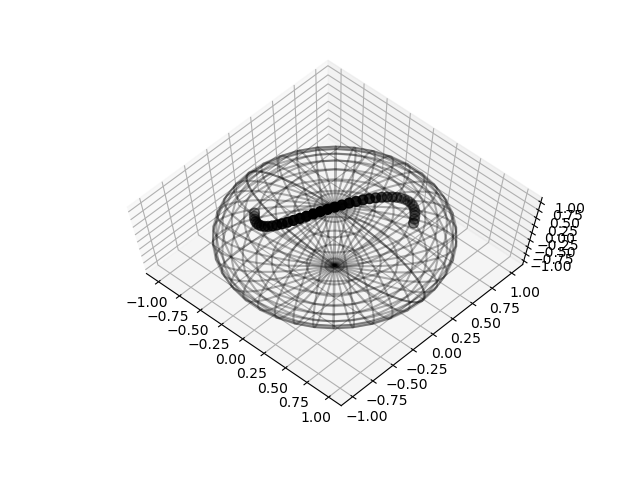
\includegraphics[scale=0.5]{Data_13.png}
        \caption{Toy data 13, $\mathbb{R}^3$}
        \label{fig:toydata}
    \end{subfigure}%
    \begin{subfigure}{.5\textwidth}
        \centering
        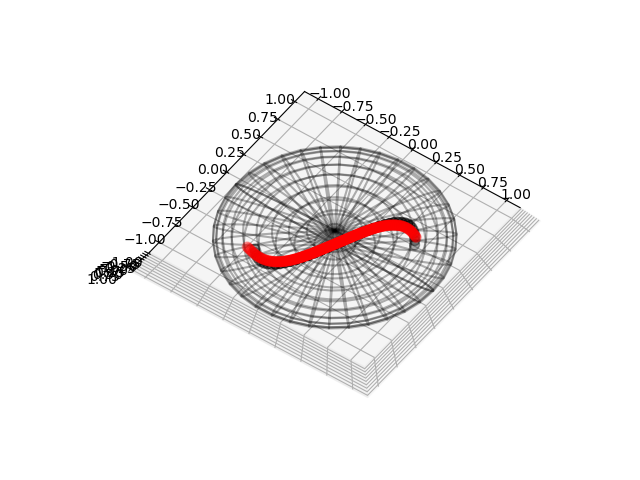
\includegraphics[scale=0.5]{single_flow_13.png}
        \caption{Principal Flow on Toy Data, $\mathbb{R}^3$}
        \label{fig:pflowtoy}
    \end{subfigure}
    \caption{Principal flow, no noise}
    \label{fig:nonnoiseflows}
\end{figure}

\newpage

For example, this dataset is created by setting the first coordinate of the 
i-th point, $x_{i, 1} = \frac{i-n/2}{n}$, then $x_{i, 2} = sin(4*x_{i, 1})/2$, 
and the third to $x_{i, 3} = \sqrt{1-x_{i, 1}^2 - x_{i, 2}^2}$, 
where n is the number of points we want to generate.\\
Now that we have seen the Toy Data, let us apply the Principal Flow 
algorithm to the data above.
This 3D plot shows the original data in black, and the principal flow in 
\textcolor{red}{red}.
With some tuning of h, the size of the neighbourhood, we can see that we have constructed
a principal flow that follows the original data almost
exactly, reconstructing an ``S" with some slight differences at the curves of the s-shape of
the original data.
We have now seen that proof that our principal flow algorithm works:
it is able to accurately reconstruct the toy data, 
the s curve on the sphere.

\subsection{With Noise}

Next, gaussian noise was added to the S-shaped data on the sphere to create a noisy dataset.
Then we fitted a principal flow to this noisy data.
\begin{figure}[ht]
\centering
\begin{subfigure}{.5\textwidth}
    \centering
    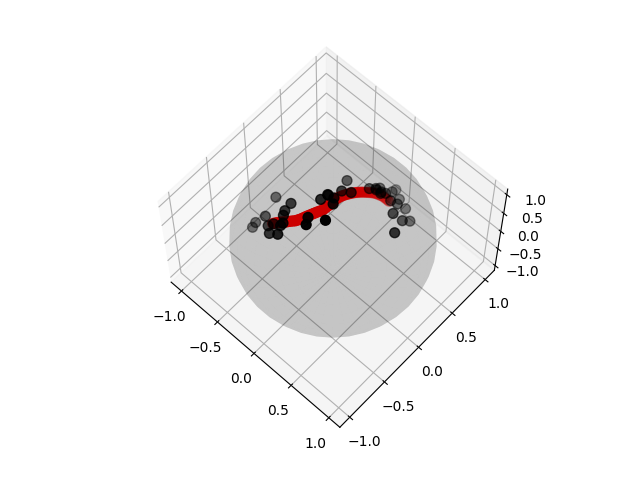
\includegraphics[scale=0.5]{noisy_13_binary.png}
    \caption{Flow on Noisy Data using binary kernel}
    \label{noisybinary}
\end{subfigure}%
\begin{subfigure}{.5\textwidth}
    \centering
    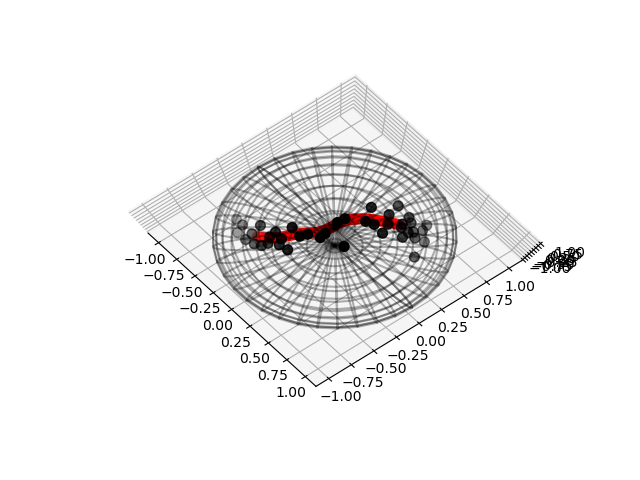
\includegraphics[scale=0.5]{noisy_13_gaussian.png}
    \caption{Flow on Noisy Data using gaussian kernel}
    \label{noisygaussian}
\end{subfigure}
\caption{Principal flow, noisy data, both kernels run with similar $h$}
\label{fig:noisyflows}
\end{figure}

We can see that the principal flow obtained seems to follow the new pattern 
of variation in the data: from the more dense cloud of points on the left, to the curve of
the points in the center to the other dense cloud of points on the right.
We can see from these examples that even with noise, our algorithm is able to discern 
the pattern of the data.

\subsection{Boundary Flow with Noise}
Next we test out our extension, our algorithm for our principal boundary.
\begin{figure}[ht]
    \begin{center}
        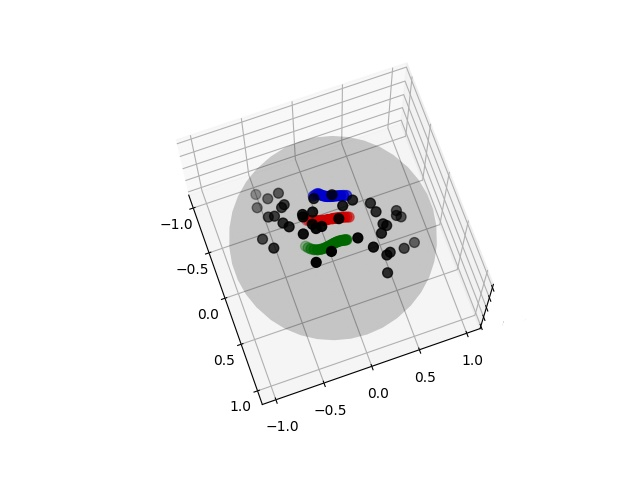
\includegraphics[scale=0.45]{noisy_boundary_flow13.jpg}
        \caption{Boundary Flow on noisy data}
        \label{fig:boundaryflows}
    \end{center}
\end{figure}\\
Since we need a ``cloud" of data, we apply some gaussian noise on the data from above,
and then run our principal boundary algorithm on it. Let the principal flow
be the curve in red, and the boundaries be in blue and green.\\
With some tuning, we obtain these three curves: we can see that the principal flow
is in the middle of the dataset, while the boundary flows accompany it in parallel
and even form to the shape of the cloud of data, bending outwards
when there is a point beyond it. Through this graph, we can see how the principal
boundary can work and be shaped by the shape of the cloud of data.

\newpage

\section{Real World Data}

Our results on artificial data are promising, however, it means little
if there are no real-world applications for our greedy principal flow. 
In this section we test our results on two real-world datasets: the MNIST dataset
and the Olivetti face dataset. Extra results are included in the appendix.

\subsection{MNIST}
 
We first test the principal flow algorithm on the MNIST dataset, a rite of passage
for machine learning algorithms. The MNIST dataset is a set of handwritten digits.
We run our principal flow algorithm using the binary kernel 
on just handwritten 3s alone.\\  
\begin{figure}[ht]
    \begin{center}
        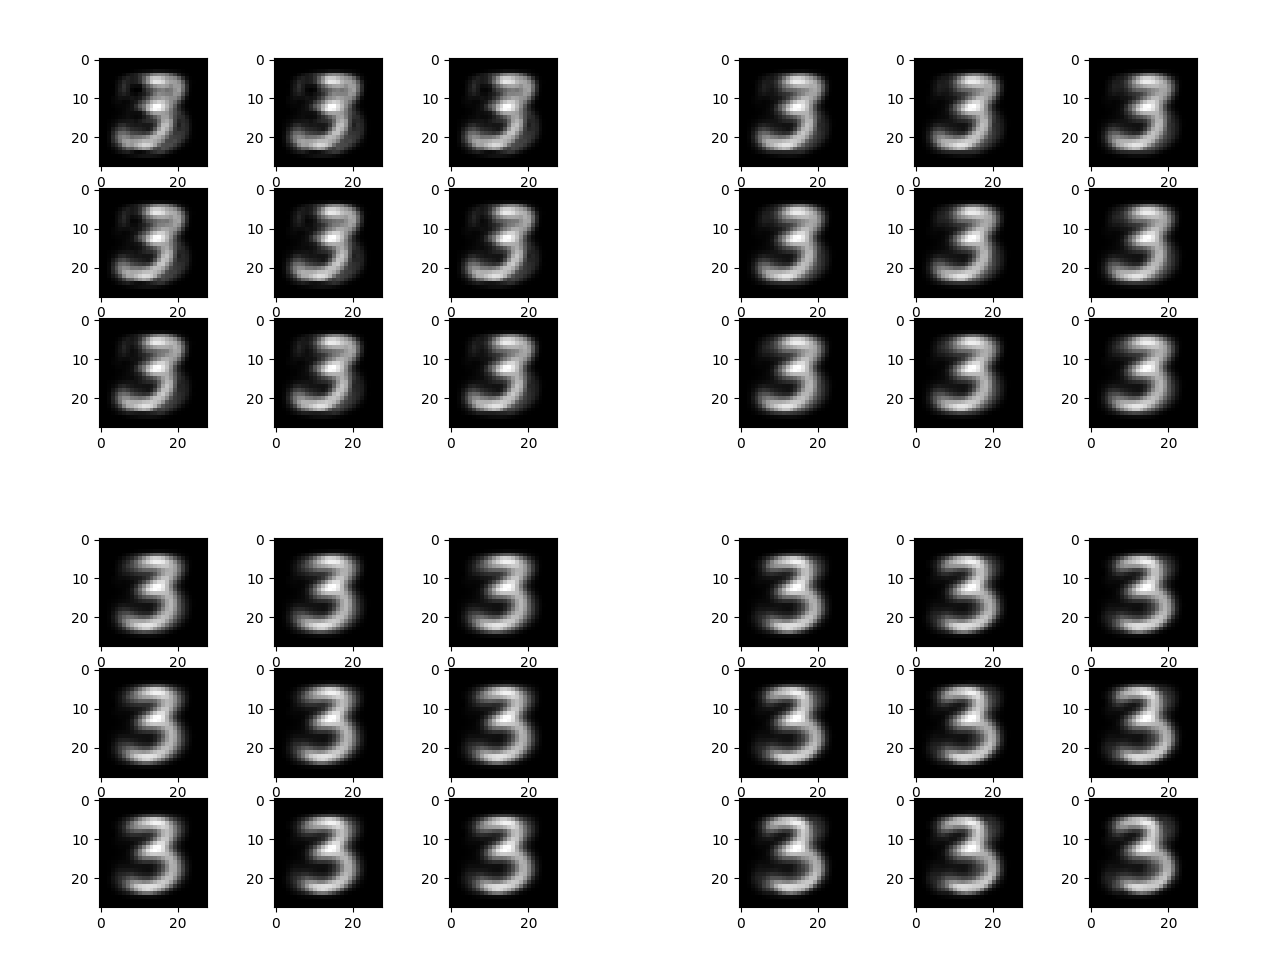
\includegraphics[scale=0.35]{main_mnist.png}
        \caption{MNIST Flows, from left to right.}
        \label{fig:mnistflows}
    \end{center}
\end{figure}
These images in the diagram below, read from left to right, 
top to bottom, are points from the greedy principal 
flow using the binary kernel. Although it does not represent 
all the variability of the 3s in the dataset, we can see that 
all the images obtained are ``nice" representations of 3s,
in that they cannot be confused with any other digit, 
and they seem to be quite neatly written.
Our principal flow algorithm obtaining these 
representations suggests that it has found some 
path through the data that has intuitive meaning: the images from this 
path are easily discernable, and seems to validate our choice of 
a hypersphere for $\mathcal{M}^d$, since data that intuitively
should be ``near" each other, such as 3s that look the same, are indeed 
close on $\mathcal{M}^d$.
Within these ``nice" 3s then we observe the source of the variability:
the slant of the digit. We can see that the digits start out 
leaning right with the upper left group of images, then slowly rotate
to slant to the left, going through a phase of being perfectly centered.
\\
This perhaps is an insight into the well-written 3s in the dataset and perhaps 
of neat handwritten digits in general: that the upper and middle part of the
digit differ mainly in orientation, while the tail remains mostly fixed.
Additionally, this gradual change in
orientation of the digit along the curve suggests that our 
greedy principal flow is able to find a central path that not only 
describes variability present in the data, but that also translates to some 
real world meaning. 
From our results from the MNIST data, 
we can see that our greedy principal flow can be used to understand
our data better, and seek out some patterns of variation
that we might otherwise be oblivious too.

\newpage
\subsection{Olivetti faces}
Next we test our algorithm on a facial dataset. The Olivetti face dataset 
is a set of 64x64 images taken between 
April 1992 and April 1994 at AT\&T Laboratories Cambridge. Although the main website 
for the dataset is no longer functioning, it can be obtained from several other 
websites. Our version was obtained from \texttt{sklearn}, a package in python.
\begin{figure}[ht]
    \begin{center}
        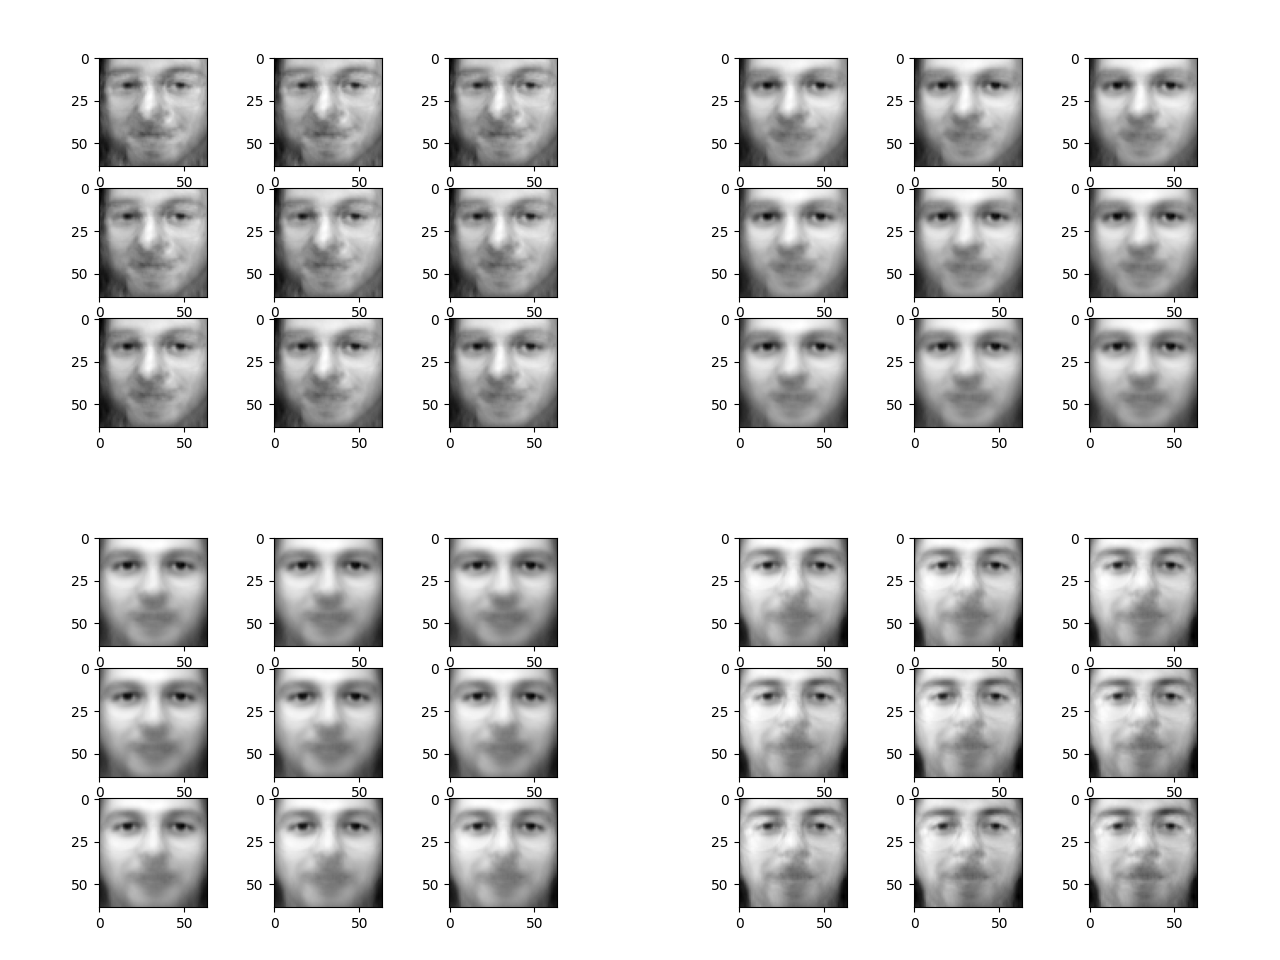
\includegraphics[scale=0.35]{main_olivetti_30_01.png}
        \caption{Flow for Olivetti face data, from left to right.}
        \label{fig:olivettiflows}
    \end{center}
\end{figure}\\
We can see that the principal flow obtained contains 
clear pictures of faces, albeit with the bottom half of their
faces slightly blurred. 
As with our results from the MNIST data,
we can glean meaning from neighbouring images on the curve:
they are close to each other in a meaningful way. This can be seen from how the set 
of faces on the upper left and some in the upper right 
are slightly tilted away from us, but gradually 
transition to facing us in the last few images of the upper right set.
These smooth transitions tell us that on $\mathcal{M}^d$,
a face slightly tilted away is near a face directly facing
the camera which makes intuitive, real world sense.
This is another indication that our choice of $\mathcal{M}^d$ does yield fruit and
preserve some real world interpretation, which validates our approach
of restricting $\mathcal{M}^d$ to the hypersphere. 
\\
Observing the images closely, we can see that 
these faces differ the most in the angle of their face,
whether they wear glasses (first few images on upper left), 
and whether they have a beard (last two images, 
bottom right and first three images, upper left).
While capturing the difference in the angle of faces in the images 
that we might not have noticed immediately is good, 
we observe that the pictures here seem to be that of only men. 
It seems like our principal flow captures the 
variability between men more so than between men and women.
However, this perhaps makes more intuitive sense:
facial images of men without glasses or a beard differ 
more from a facial image of a man with these features than
an image of a woman's face would.
Through our results here, we can see that while our greedy principal flow
incorporates mostly local information (i.e the faces in some neighbourhood around 
our current flow point), the flow obtained is also open to a more global interpretation: 
we can see the faces transition through different angles, 
tilting in the same direction continuously, 
and watch as it describes to us the main sources of variation in the data set. 

\chapter{Future Directions}

The topic of principal flows and manifold learning in general is a rich field 
with much potential, and there are many avenues of 
expanding the work done in this report. 
One potential direction is constructing the $k$-th order principal flows, where $k>1$. 
Another potential avenue of research is using different kinds of $\mathcal{M}^d$. 
In this report, we have restricted ourselves only to the hypersphere. Although this 
might be a ``good enough" approximation, if we had intuition about the specific form 
of the manifold on which our multivariate data lies, and we determine that the 
hypersphere is unsuitable, then this current principal flow would not be able to 
accomodate this intuition. With a different manifold, we might be able to obtain 
a different principal flow that might give us more information about the 
variability of the data and describe it more appropriately than using the hypersphere. 
Additionally, we could also extend the greedy principal boundary to be a maximal margin
classifier. Although this has already been done in \cite{principalboundary}, 
it has yet to be done with a greedy approach, and would be the first
greedy maximal margin classifier for multivariate data lying on some 
Riemannian manifold.

\addcontentsline{toc}{chapter}{Bibliography}
\begin{thebibliography}{9}


\bibitem{mds}
Borg, I., and Groenen, P. J. F. (2005),
\textit{Modern Multidimensional Scaling, Theory and Applications}, 
2 edn Springer.

\bibitem{pca2}
Jollife, I. T. (2002). \textit{Principal Component Analysis}, 
2 edn Springer.

\bibitem{pca}
Pearson, K. (1901). ``On Lines and Planes of Closest Fit to Systems of Points in Space". 
\textit{Philosophical Magazine}. 2 (11): 559–572.

\bibitem{pga}
Fletcher, P. T., Lu, C., Pizer, S. M., and Joshi, S. (2004), 
``Principal Geodesic Analysis for the Study of Nonlinear Statistics of Shape," 
\textit{IEEE Transactions on Medical Imaging}, 23, 995-1005.

\bibitem{isomap}
Tenenbaum, J. B., Silva, V. D., and Langford, J. C. (2000). ``A Global
Geometric Framework for Nonlinear Dimensionality Reduction," 
\textit{Science}, 290, 2319-2323.

\bibitem{principalboundary}
Yao, Z., and Zhang, Z. (2019) ``Principal Boundary on Riemannian Manifolds," 
\textit{Journal of the American Statistical Association} 115(531), 1435–1448.

\bibitem{principalflow}
Panaretos, V. M., Pham, T., and Yao, Z. (2014), 
``Principal Flows" \textit{Journal of the American
Statistical Association}, 109, 424-436.

\bibitem{ancient}
Thorpe, J. A. (1979). \textit{Elementary Topics in Differential Geometry},
Springer.

\bibitem{lle}
Roweis, S. T., and Saul, L. K. (2003). ``Think Globally, Fit Locally:
Supervised Learning of Low Dimensional Manifolds.” \textit{Journal of Machine
Learning Research}, 4, 119–155.

\end{thebibliography}

\begin{appendices}
\chapter{Extra Results from the Principal Flow}

\section{Fashion MNIST}
\begin{figure}[ht]
    \begin{center}
        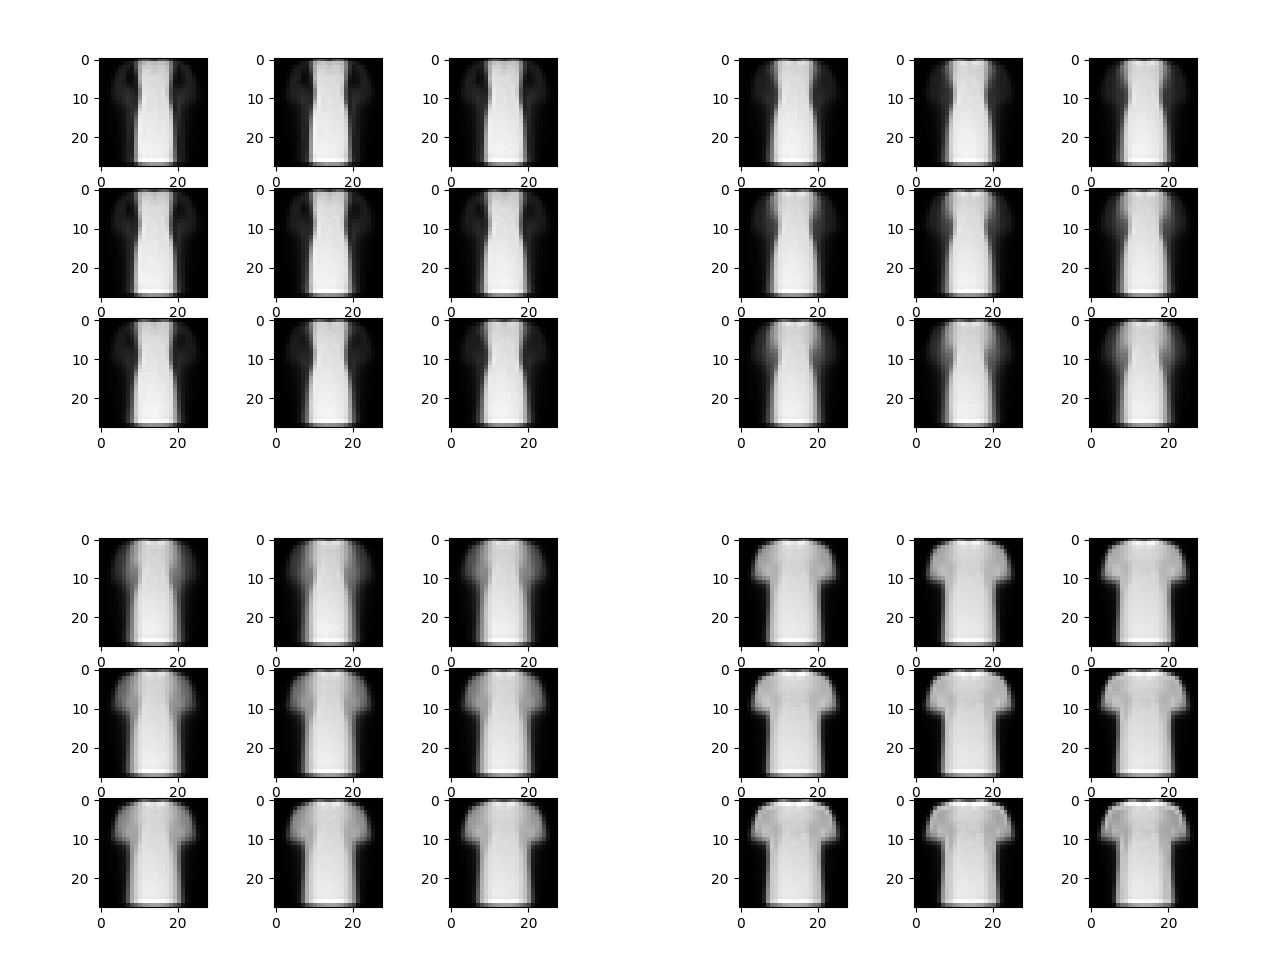
\includegraphics[scale=0.3]{main_fashion.png}
        \caption{Fasion MNIST Flows, from left to right.}
        \label{fig:fashionmnistflows}
    \end{center}
\end{figure}
Here we test our principal flow on objects, and rather on 2 pieces of fashion that
look quite alike: t-shirts and dresses.
Here we can watch as dresses morph into t-shirts. More than just an interesting graphic,
it shows that the principal flow is able to capture the variability of the data:
here the data varies very clearly in the outline of the images, and images on the
principal flow reflect this main source of variability.

\section{Cartoon Faces}
Now we test our principal flow on a dataset of cartoon faces.
\begin{figure}[ht]
    \begin{center}
        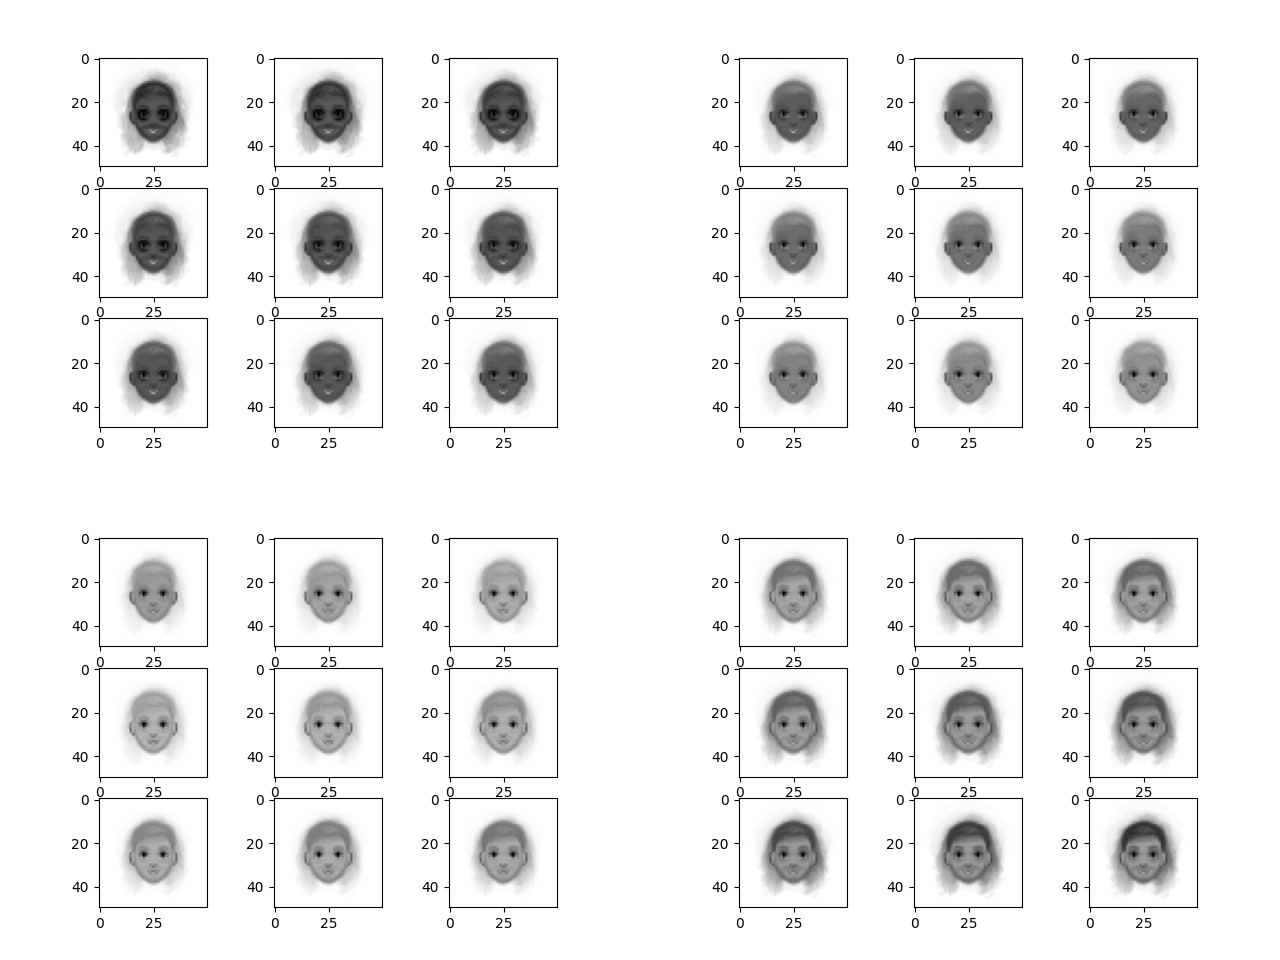
\includegraphics[scale=0.25]{main_cartoon_10_01.png}
        \caption{Cartoon face Flows, from left to right.}
        \label{fig:cartoonfaceflows1}
    \end{center}
\end{figure}

When run on a dataset of cartoon faces, the principal flow finds a series of 
faces that differ greatly in skin color and in hair color. Along the flow 
we can see that the faces start with a dark skin color and gradually 
transition to a lighter skin color, then get darker along with their hair color. 
Here we can see that faces vary mainly on skin tone and hair color, which makes intuitive sense, 
since other features like spectacles and a particular hair shape may not feature on many
data points.

\newpage
\section{Faces in the Wild}
\begin{figure}[ht]
    \begin{center}
        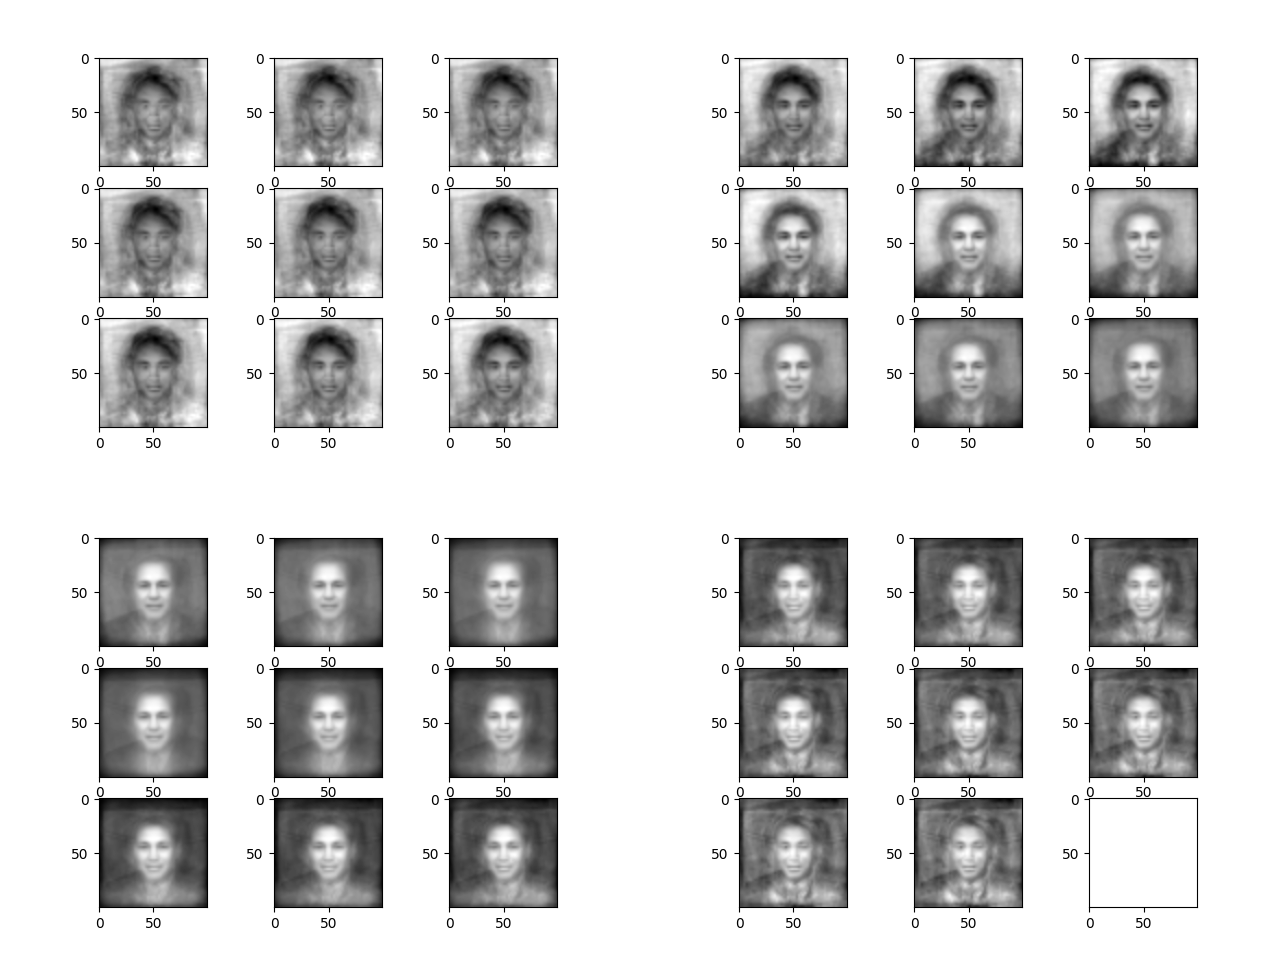
\includegraphics[scale=0.3]{main_lfw_10_05.png}
        \caption{Faces in the wild flow, from left to right.}
        \label{fig:Facesinthewildflows}
    \end{center}
\end{figure}
Here we test our principal flow algorithm on real faces with differing backgrounds, 
since these are photos found online. As with the cartoon faces, we can see that
these faces differ in skin tone but also in eyebrow color, eye shape and background. 
This makes sense, since skin tone will determine a large portion of the face,
and the background also takes up a large part of the images, and are likely to differ 
quite greatly.
\end{appendices}


\end{document}